\section{Shell Elements}\label{sec:Shell}
 Shell elements are used when structures need to be modeled where plane stresses as well as bending stresses are present. Different types of shell elements are available, including curved shell elements, shells of revolution, generalized shells or flat shell elements~\cite{cook2002concepts}. The flat shell elements are subject of this work. Such an element can be constructed by the superposition of a plane and a plate element. This section contains the fundamentals of linear elastic problems - the field of application for the shell element - as well as the mathematical derivation of the plane and plate element, their combination resulting in the shell element and the necessary coordinate transformation that is needed for the implementation. 
 
 
 \subsection{Introduction to Linear Elastic Problems}\label{sec:Shell-IntroLinEla}
 In the following the fundamental equations of linear elasticity will be considered. Here, the spatial case is used for demonstration, but every lower dimensional problem can easily be derived from it.
 The following definitions will be used in this thesis:
 \begin{align}
 \vec{u} &= \begin{pmatrix}
 u & v & w
 \end{pmatrix}^T \text{displacement\ vector}\\
 \vec{f} &= \begin{pmatrix}
 f_x & f_y & f_z
 \end{pmatrix}^T \text{external\ force\ vector}
 \end{align}
 The strains and stresses can either be described in form of tensors $\underline{\varepsilon}$ and $\underline{\sigma}$, or as vectors $\vec{\varepsilon}$ and $\vec{\sigma}$:
 \begin{align}
 \underline{\varepsilon} &= \begin{pmatrix}
 \varepsilon_{xx} & \varepsilon_{xy} & \varepsilon_{xz} \\
 \varepsilon_{yx} & \varepsilon_{yy} & \varepsilon_{yz} \\
 \varepsilon_{zx} & \varepsilon_{zy} & \varepsilon_{zz} \end{pmatrix}\\
 \underline{\sigma} &= \begin{pmatrix}
 \sigma_{xx} & \sigma_{xy} & \sigma_{xz} \\
 \sigma_{yx} & \sigma_{yy} & \sigma_{yz} \\
 \sigma_{zx} & \sigma_{zy} & \sigma_{zz} \end{pmatrix}
 \end{align}
 \begin{align}
 \vec{\varepsilon} &= \begin{pmatrix}
 \varepsilon_{xx} & \varepsilon_{yy} & \varepsilon_{zz} & 2\varepsilon_{xy} & 2\varepsilon_{yz} & 2\varepsilon_{zx} \end{pmatrix}^T\\
 \vec{\sigma} &= \begin{pmatrix}
 \sigma_{xx} & \sigma_{yy} & \sigma_{zz} & \sigma_{xy} & \sigma_{yz} & \sigma_{zx} \end{pmatrix}^T
 \end{align}
 In the case of isotropic materials the strains and stresses are symmetrical, i.e. $\varepsilon_{xy} = \varepsilon_{yx}, \varepsilon_{xz} = \varepsilon_{zx}, \varepsilon_{yz} = \varepsilon_{zy}$ and $\sigma_{xy} = \sigma_{yx}, \sigma_{xz} = \sigma_{zx}, \sigma_{yz} = \sigma_{zy}$. As stated in~\cite{steinke2005finite}, the relation between displacements and strains is as follows:
 \begin{align}\label{eq:displ_strain_relation}
 \underline{\varepsilon} &= \frac{1}{2}\left(\nabla\vec{u} + \vec{u}\:\nabla \right) \\
 \vec{\varepsilon} &= \underline{L}\vec{u} \nonumber
 \end{align}
 Equation \eqref{eq:displ_strain_relation} relates the displacement vector field $\vec{u}$ with the strain field $\underline{\varepsilon}$, or $\vec{\varepsilon}$ respectively. Here, $\underline{L}$ is a differential operator. This strain-displacement relation is also called \textit{kinematic relationship}~\cite{steinke2005finite}.
 
 In general, initial strains can exist inside the material, for example due to temperature changes or shrinkage. Such initial strains are denoted by $\vec{\varepsilon_0}$ and the stresses will be influenced by the difference between the current and initial strains. Additionally, one can imagine initial residual stresses $\vec{\sigma_0}$ that can be added to the general equation:
 \begin{equation}\label{eq:stress-strain-relation}
 \vec{\sigma} = \underline{D}\left(\vec{\varepsilon}-\vec{\varepsilon_0}\right)+\vec{\sigma_0}
 \end{equation}
 where $\underline{D}$ is the material matrix. In the simplest case of linear elasticity with isotropy, $\underline{D}$ only contains of two parameters, namely the elastic modulus $E$ (also known as the Young's modulus) and the Poisson's ratio $\nu$. The former one defines the relationship between the stress and strain in a material, the latter one results as the quotient of the fraction of expansion and the fraction of compression for small changes.
 
 In the following the initial conditions are excluded, resulting in the a simpler form of equation \eqref{eq:stress-strain-relation}:
 \begin{equation}
 \vec{\sigma} = \underline{D}\ \vec{\varepsilon}
 \end{equation}
 For the said isotropic case, $\underline{D}$ results in~\cite{zienkiewicz2000finite}:
 \begin{equation}
 \underline{D} = \frac{E}{1-\nu^2}\begin{pmatrix}
 1 & \nu & 0 \\
 \nu & 1 & 0 \\
 0 & 0 & \frac{1-\nu}{2}
 \end{pmatrix}
 \end{equation}
 
 The equilibrium conditions as described in~\cite{steinke2005finite}, are as follows:
 \begin{equation}\label{eq:equilibrium-conditions}
 \underline{L} \vec{\sigma} + \vec{b} = \vec{0}
 \end{equation}
 where the vector $\vec{b}$ describes internal volume forces and $\vec{0}$ is the zero vector.
 
 Two different boundary conditions are distinguished: Essential and natural boundary conditions. The first one is geometrically described. An initial displacement $\vec{u^0}$ is impressed on a surface part $\Omega_u$ of the object:
 \begin{equation}
 \vec{u} = \vec{u^0}\quad \text{on}\quad \Omega_u
 \end{equation}
 The natural boundary conditions are represented by force conditions. They can be described as follows:
 \begin{equation}
 \underline{n} \vec{\sigma} = \vec{p^0}\quad \text{on}\quad \Omega_p
 \end{equation}
 where the matrix $\underline{n}$ contains entries of the object boundary's normal vector, $\vec{p^0}$ described the edge stress and $\vec{\sigma}$ is the stress vector:
 \begin{align}
 \vec{n} &= \begin{pmatrix}
 n_x\\n_y\\n_z
 \end{pmatrix}\\
 \underline{n} &= \begin{pmatrix}
 n_x & 0 & 0 & n_y & 0 & n_z\\
 0 & n_y & 0 & n_x & n_z & 0\\
 0 & 0 & n_z & 0 & n_y & n_x
 \end{pmatrix}
 \end{align}
 
 In~\cite{steinke2005finite} the principle of the total potential for the fundamental equations of linear elasticity is illustrated. Initial point is the weak formulation of the equilibrium conditions \eqref{eq:equilibrium-conditions} for a body $V$:
 \begin{equation}
 \int_{V} \left(\underline{L} \vec{\sigma} + \vec{b}\right) \vec{\lambda}\ dV = 0
 \end{equation}
 The introduction of Lagrange multipliers $\vec{\lambda}$ lead to a weighting and can be expressed as variation of $\delta \vec{u} = \vec{\lambda}$. The result of the derivation of the above equation is the expression of the total potential $\Pi$:
 \begin{equation}
 \Pi = \frac{1}{2} \int_{V} \vec{\sigma}^T \vec{\varepsilon}\ dV - \left(\int_{V}\vec{b}^T \vec{u}\ dV - \int_{\Omega_p} \vec{p^0}^T \vec{u}\ d\Omega_p\right) = \Pi_D - \Pi_e
 \end{equation}
 The first term describes the elastic deformation energy $\Pi_D$, the two terms in brackets combine the potential of the external forces $\Pi_e$
 
 \subsection{Plane Element}\label{sec:Shell-Plane}
  Plane elements are characterized by that loads are only applied in mid-surface directions of an element and all displacements, strains and stresses happen in the mid-surface, too. In this section plane elements are discussed in more detail and two different element types, a three-node triangular element and a four-node quadrilateral element, are described.
  
  
  \subsubsection{Problem Definition}\label{sec:Shell-Plane-ProbDef}
  \begin{figure}[htbp]%- Bild ähnlich ch7.1 mit xy-Ausdehnung, Dicke t, Mittelfläche, Rand, KoSys; Streckenlast q0 und Volumenkraft g aber weglassen
\centering
%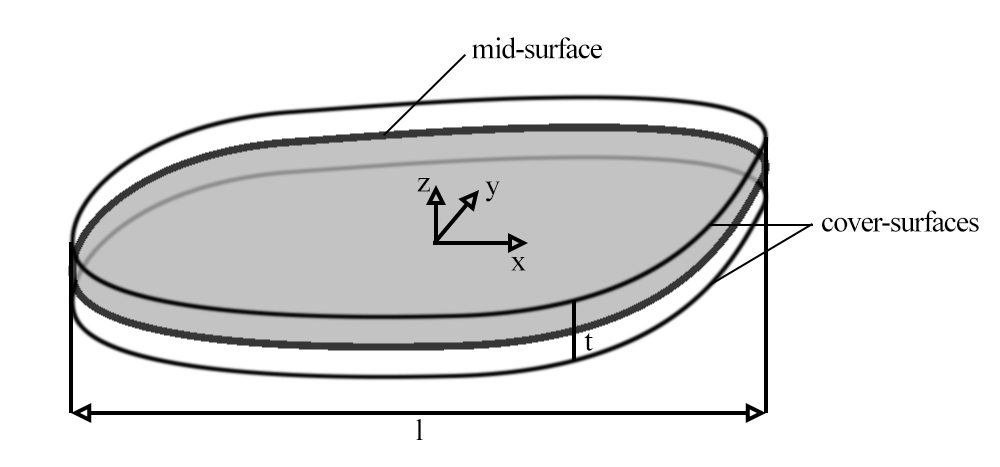
\includegraphics[width=0.97\linewidth]{figures/plane}
\setlength\unitlength{1.0cm}
\begin{picture}(12,6)
\thinlines
\put(0,0){\pgfsetfillopacity{1.0}\Curve(0.5,2.5)<0,0.25>(3.5,4.25)<1,0.125>(7.5,4.5)<1,0>(10,2.5)<-1,-1>(6,1)<-0.5,-0.05>(2.5,1)<-0.5,0.125>(0.5,2.5)<0,0.5>}
\thicklines
{\pgfsetfillopacity{0.8}\color{gray}\Curve*(0.5,3)<0,0.25>(3.5,4.75)<1,0.125>(7.5,5)<1,0>(10,3)<-1,-1>(6,1.5)<-0.5,-0.05>(2.5,1.5)<-0.5,0.125>(0.5,3)<0,0.5>}
\put(0,0){\pgfsetfillopacity{1.0}\color{black}\Curve(0.5,3)<0,0.25>(3.5,4.75)<1,0.125>(7.5,5)<1,0>(10,3)<-1,-1>(6,1.5)<-0.5,-0.05>(2.5,1.5)<-0.5,0.125>(0.5,3)<0,0.5>}
\put(6.6,2.9){$x$}
\put(5.5,3){\vector(1,0){1}}
\put(6.1,3.4){$y$}
\put(5.5,3){\vector(0.5,0.65){0.5}}
\put(5.4,4.1){$z$}
\put(5.5,3){\vector(0,1){1}}
\thinlines
\put(0,0){\pgfsetfillopacity{1.0}\Curve(0.5,3.5)<0,0.25>(3.5,5.25)<1,0.125>(7.5,5.5)<1,0>(10,3.5)<-1,-1>(6,2)<-0.5,-0.05>(2.5,2)<-0.5,0.125>(0.5,3.5)<0,0.5>}
\Dline(0.5,3.5)(0.5,0.5){0.1}
\Dline(10.37,3.5)(10.37,0.5){0.1}
\put(5,0.5){\vector(-4.5,0){4.5}}
\put(5,0.5){\vector(5.37,0){5.37}}
\put(5.4,0.15){$l$}
\Line(2.5,2)(2.5,1)\put(2.43,0.7){$t$}
\polyline(10,3.5)(11,3)(10,2.5)\put(11.1,2.9){cover-surfaces}
\Line(7.5,5)(9.5,5.5)\put(9.6,5.4){mid-surface}
\end{picture}
\caption{Schematic view of a plane object with main dimension $l$ and thickness $t$. The two cover-surfaces are located at $z=\pm \frac{t}{2}$, the mid-surface at $z=0$.}
\label{fig:plane}
\end{figure}
  In Figure~\ref{fig:plane} an object is shown which extends to the x and y axis as its primary direction. The extend in z-direction is smaller and denoted by thickness $t$. The mid-surface located in between the top and bottom surface areas has the coordinate $z=0$. Its local z-axis equals the normal vector of the mid place. In the following, such an object is called \textit{plane}.
  
  %- Bed. für ebenen Spannungszustand (eb. Dehnungszustand erwähnen und auf Ref (z.B. Zienkiewicz) verweisen)
  There are two different formulations regarding plane elements: Plane stress and plane strain. The directions of displacements $u$ and $v$ along the orthogonal local x and y axis defining its displacement field is a common feature of both problems. Also, both have in common, that only strains and stresses in the xy-plane have to be considered: Instead of nine, only three components remain. While in the case of plane stress all other stress components are zero, in plane strain the stress in direction perpendicular to the xy-plane is non-zero. In this thesis only plane stress will be discussed in further detail. More information about plane strain is given in~\cite{zienkiewicz2000finite} and~\cite{braess2007finite}, for instance.
  The following conditions must be satisfied, such that a plane can be in \textit{plane stress}~\cite{steinke2005finite}:
  \begin{itemize}
  	\item The thickness $t$ varies only slightly and it must hold: $t/l \ll 1$, with $l$ the extent of the larger side of the plane element.
  	\item The load is applied to the mid-surface.
  	\item Displacements, strains and stresses are constant across the thickness.
  \end{itemize}
  The stress components $\sigma_{xz},\sigma_{yz},\sigma_{zz}$ normal to the surface areas with $z \pm t/2$ vanish (equals zero). Therefore only the two normal stress components $\sigma_{xx}$ and $\sigma_{yy}$ and the transverse stress component $\sigma_{xy}$ are left non-zero.
    
  %- Verschiebungen, Dehnungen und Spannungen beschreiben + kinematische Beziehung + Stoffgleichung\newline
  Displacements can only occur in x and y direction. $u$ will be the displacement along x and $v$ along y. The displacement field $\vec{u}$ is as follows:
  \begin{equation}
  \vec{u}=\begin{pmatrix}
  u(x,y) & v(x,y)
  \end{pmatrix}^T
  \end{equation}
  The vector for the strain components:
  \begin{equation}
  \vec{\varepsilon}=\begin{pmatrix}
  \varepsilon_{xx} & \varepsilon_{yy} & 2\varepsilon_{xy}
  \end{pmatrix}^T
  \end{equation}
  Sometimes $2\varepsilon_{xy}$ is shortened to $\gamma_{xy}$~\cite{steinke2005finite}.
  The vector holding the stress components is similar to that of the strain vector:
  \begin{equation}
  \vec{\sigma}=\begin{pmatrix}
  \sigma_{xx} & \sigma_{yy} & \sigma_{xy}
  \end{pmatrix}^T
  \end{equation}
  The kinematic relationship $\vec{\varepsilon}=\underline{L}\vec{u}$ (eq. \eqref{eq:displ_strain_relation}) linking the displacements $\vec{u}$ with the strains $\vec{\varepsilon}$ can be written at full length:
  \begin{equation}\label{eq:t3displ-str-rel}
  \vec{\varepsilon} = \begin{pmatrix}
  \varepsilon_{xx} \\
  \varepsilon_{yy} \\
  2\varepsilon_{xy}
  \end{pmatrix} =
  \begin{pmatrix}
  \frac{\partial u}{\partial x} \\
  \frac{\partial v}{\partial y} \\
  \frac{\partial u}{\partial y} + \frac{\partial v}{\partial x}
  \end{pmatrix} =
  \begin{pmatrix}
  \frac{\partial}{\partial x} & 0 \\
  0 & \frac{\partial}{\partial y} \\
  \frac{\partial}{\partial y} & \frac{\partial}{\partial x}
  \end{pmatrix}
  \begin{pmatrix}
  u \\
  v
  \end{pmatrix}
  = \underline{L} \vec{u}
  \end{equation}
  With the strains known and considering equation \eqref{eq:displ_strain_relation}, one can calculate the stresses $\vec{\sigma}$:
  \begin{equation}\label{eq:sigma=D*eps}
  \vec{\sigma} = \begin{pmatrix}
  \sigma_{xx} \\
  \sigma_{yy} \\
  \sigma_{xy}
  \end{pmatrix} = \frac{E}{1-\nu^2} \begin{pmatrix}
  1 & \nu & 0 \\
  \nu & 1 & 0 \\
  0 & 0 & \frac{1-\nu}{2}
  \end{pmatrix} \begin{pmatrix}
  \varepsilon_{xx} \\
  \varepsilon_{yy} \\
  2\varepsilon_{xy}
  \end{pmatrix} = \underline{D} \vec{\varepsilon} = \underline{D}\; \underline{L} \vec{u}
  \end{equation}
  %- Randbedingungen: q0 Streckenlast beschreiben, aber angeben, dass sie hier nicht beachtet werden, punktf. Ladungen werden hier benutzt\newline

  After Steinke~\cite{steinke2005finite}, the essential boundary conditions $\vec{u} = \vec{u^0}$ and the natural boundary conditions $t\ \underline{n}\ \vec{\sigma} = \vec{q^0}$ will be applied onto the objects boundary $\Gamma$, with $t$ being the object's thickness and $\vec{q^0}$ representing an edge load. The matrix $\underline{n}$ looks as follows~\cite{steinke2005finite}:
  \begin{equation}
  \underline{n} = \begin{pmatrix}
  n_x & 0 & n_y\\ 0 & n_y & n_x
  \end{pmatrix}
  \end{equation}
  Beside line loads, nodal forces $\vec{F} = \begin{pmatrix}
  F_x & F_y
  \end{pmatrix}^T$ are also possible.
  
  The total potential of the plane element problem looks as follows~\cite{steinke2005finite}:
  \begin{equation}
  \Pi = \frac{1}{2} \int_{V}\vec{\varepsilon}^T\vec{\sigma}dV - \int_{V} \vec{u}^T \vec{b}\ dV - \int_{\Gamma_q}\vec{u}^T \vec{q}\ d\gamma -\vec{u}^T \vec{F}
  \end{equation}
  The first term describes the elastic strain energy, the last three terms describe the different external forces. The first of the three describes the potential of the volume forces $\vec{b}^T = \rho \begin{pmatrix}
  g_x & g_y
  \end{pmatrix}$, where $\rho$ is the object's density and $g_x, g_y$ represents accelerations in the two directions. The second term stands for the line load along an edge $\Gamma_q$ and the last term contains the single nodal forces.
  
  The external forces are summarized in this work to the last term only. Line loads and volume forces can be converted to nodal load, assuming a linear distribution over the edges and the interior of the element, respectively~\cite{steinke2005finite}. Therefore, the total potential of the plane element shrinks to the following:
  \begin{equation}\label{eq:planeFunctional}
  \Pi = \frac{1}{2} \int_{V}\vec{\varepsilon}^T\vec{\sigma}dV - \vec{u}^T \vec{F}
  \end{equation}
  
  
  
  
  
  
  
  
  \subsubsection{Tri-3 Plane Element}\label{sec:Shell-Plane-Tri}
  In Section~\ref{sec:Shell-Plane-ProbDef} the plane element's functional was derived (eq. \eqref{eq:planeFunctional}). Now, the focus is on the functional discretization. The constructed finite element will be a three-node triangular element in the following also denoted as \textbf{Tri-3}. Figure~\ref{fig:plane_triangulation} shows a general, planar object defined to be placed in the xy-plane. The first discretization step is to divide the object into single triangles approximating the shape of it. This process is called triangulation. Every one of these triangles then represents a finite element with one node at every corner. The finer the triangulation is done the better the object and its boundary are matched by its discrete complement, but also the more finite elements have to be considered in later calculations.
  \begin{figure}[htbp]% Bild von trianguliertem Körper
    	\centering
    	%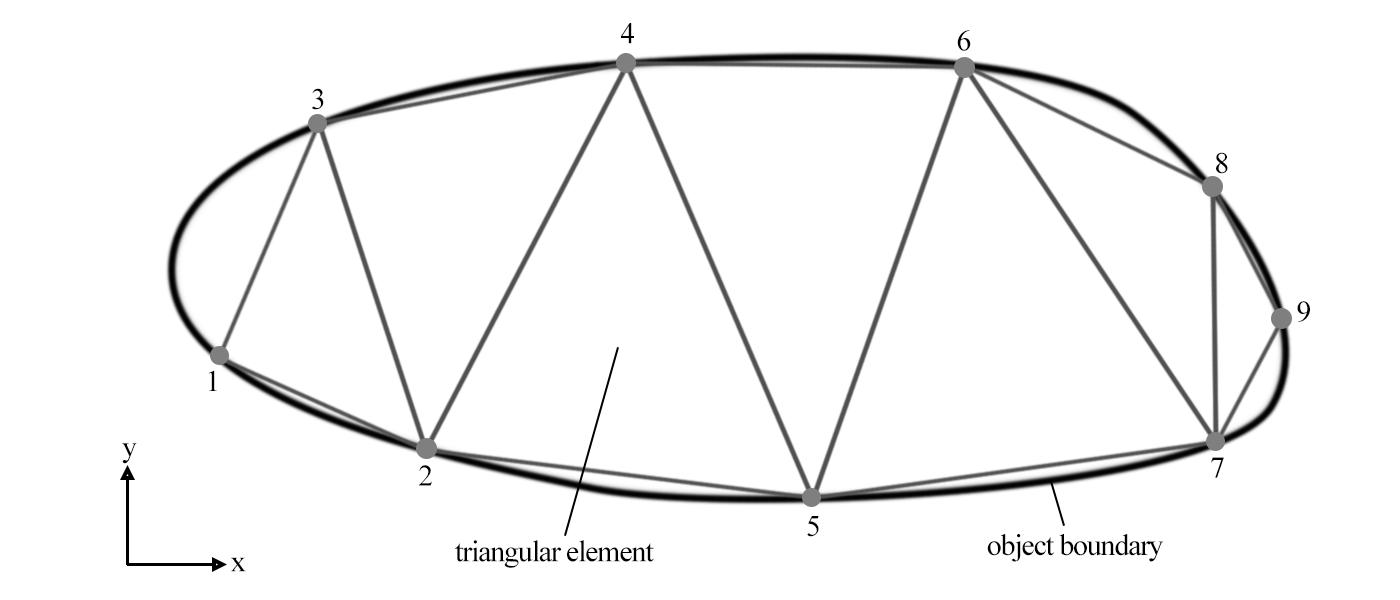
\includegraphics[width=1.0\linewidth]{figures/plane_triangulation}
    	\setlength\unitlength{0.9cm}
    	\begin{picture}(14,6)
    	\thicklines
    	\put(0.2,0.1){\vector(1,0){1.5}}
    	\put(0.2,0.1){\vector(0,1){1.5}}
    	\put(1.8,0){$x$}
    	\put(0.1,1.7){$y$}
    	
    	\put(1, 2.5){\cbezier(0,0)(0,0.5)(0.5,1.5)(2,2)}
    	\put(3,4.5){\cbezier(0,0)(1.5,0.5)(2.5,0)(3,0.5)}
    	\put(6,5){\cbezier(0,0)(0.5,0.5)(1.5,0.5)(3.5,0.5)}
    	\put(9.5,5.5){\cbezier(0,0)(2,0)(3,-1)(3.5,-2)}
    	\put(13,3.5){\cbezier(0,0)(0.5,-1)(-0.5,-2)(-2,-2)}
    	\put(11,1.5){\cbezier(0,0)(-1.5,0)(-2.5,0.5)(-3.5,1)}
    	\put(7.5,2.5){\cbezier(0,0)(-1,0.5)(-2.5,0)(-3.5,-1)}
    	\put(4,1.5){\cbezier(0,0)(-1,-1)(-3,0.5)(-3,1)}
    	\thinlines
    	\polyline(1,2.5)(3,4.5)(6,5)(9.5,5.5)(13,3.5)(11,1.5)(7.5,2.5)(4,1.5)(1,2.5)
    	\polyline(3,4.5)(4,1.5)(6,5)(7.5,2.5)(9.5,5.5)(11,1.5)(13,3.5)
    	\put(0.5,5.5){object boundary} \polyline(2,5.2)(1.65,3.7)
    	\put(6,1){triangular element} \polyline(8,1.5)(9.2,3)
    	\put(0.6,2.3){$1$}
    	\put(4.0,1.1){$2$}
    	\put(2.85,4.6){$3$}
    	\put(7.3,2.1){$4$}
    	\put(5.8,5.1){$5$}
    	\put(9.4,5.6){$6$}
    	\put(10.85,1.05){$7$}
    	\put(13.2,3.4){$8$}
    	\end{picture}
    	\caption{A plane object is partitioned into several triangular elements. This process is called triangulation.}
    	\label{fig:plane_triangulation}
  \end{figure}
    
  \begin{figure}[htbp]
  	\centering
  	%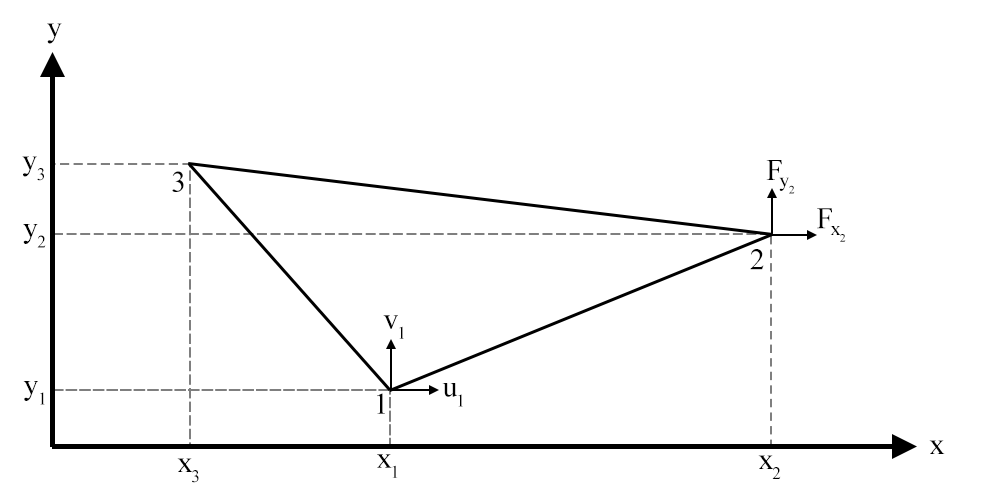
\includegraphics[width=1.0\linewidth]{figures/plane_triangle}
  	\setlength\unitlength{0.9cm}
	\begin{picture}(14,6)
	\thicklines
	\put(0.4,0.3){\vector(1,0){13.5}}
	\put(0.4,0.3){\vector(0,1){5.5}}
	\put(14.0,0.2){$\mathbf{x}$}
	\put(0.3,5.9){$\mathbf{y}$}
	
	\put(6.2,0.7){\line(6,2.5){6}}
	\put(5.85,0.35){$1$}
	\put(12.2,3.2){\line(-10,1){10}}
	\put(12.3,2.8){$2$}
	\put(2.2,4.2){\line(4,-3.5){4}}
	\put(1.9,3.8){$3$}
	
	\thinlines
	\Dline(6.2,0.7)(6.2,0.3){0.1}
	\put(6,0){$x_1$}
	\Dline(6.2,0.7)(0.4,0.7){0.1}
	\put(0,0.6){$y_1$}
	\Dline(12.2,3.2)(12.2,0.3){0.1}
	\put(12,0){$x_2$}
	\Dline(12.2,3.2)(0.4,3.2){0.1}
	\put(0,3.1){$y_2$}
	\Dline(2.2,4.2)(2.2,0.3){0.1}
	\put(2,0){$x_3$}
	\Dline(2.2,4.2)(0.4,4.2){0.1}
	\put(0,4){$y_3$}
	
	\put(6.2,0.7){\vector(1,0){1}}
	\put(7.3,0.6){$u_1$}
	\put(6.2,0.7){\vector(0,1){1}}
	\put(6.0,1.8){$v_1$}
	
	\put(12.2,3.2){\vector(1,0){1}}
	\put(13.3,3.1){$F_{x_2}$}
	\put(12.2,3.2){\vector(0,1){1}}
	\put(12.0,4.3){$F_{y_2}$}
	\end{picture}
  	\caption{A three-node triangular element is shown with its coordinates projected onto the axes. For the first node its nodal displacements and for the second node its nodal forces are exemplarily illustrated.}
  	\label{fig:plane_triangle}
  \end{figure}
    
  One triangular finite element is shown in Figure~\ref{fig:plane_triangle}. It is defined by the coordinates $(x_i,y_i)$ of its three nodes. Since the element is located in the xy-plane, the z-coordinate is of no interest and will be ignored. At every node, forces can be applied denoted with $F_{x_i}$ and $F_{y_i}$. Accordingly, every node can be displaced. The movement along the x-axis is denoted with $u_i$ and with $v_i$ along the y-axis, respectively. Note, that the node numbering is in anti-clockwise direction. This convention will be kept throughout the thesis, and is important when implementing the FEM code.
  In this thesis only triangles defined by three nodes are discussed. There are many more finite elements forming triangles, such as six-node triangles or even seven-node triangles. The main difference between these types of elements are the order of shape functions. More details about higher order triangular finite elements can be found in \cite{zienkiewicz2000finite}, \cite{bergan1985triangular}, \cite{cook2002concepts}, \cite{braess2007finite}.
  
  % ansatzfunktion (abgewandelt statt phi, u und v separat)\\
  In the case of a three-node triangle the test functions for the two displacements $u$ and $v$ are the same and thus $u$ and $v$ can be replaced by an arbitrary function $\psi$\cite{steinke2005finite}:
  \begin{align}\label{eq:t3_ansatz}
  \psi(x,y) &= a_0 + a_1L_1 + a_2L_2 = \begin{pmatrix}
  1 & L_1 & L_2
  \end{pmatrix} \begin{pmatrix}
  a_0 \\ a_1 \\ a_2
  \end{pmatrix} = \vec{x}^T \vec{a}
  \end{align}
  defined in triangular coordinates (see Figure~\ref{fig:tri_coords}).
  
  \begin{figure}[htbp]% dreieckskoordinaten (ähnlich bild 2.7 auf s.39(53))
  	\centering
  	%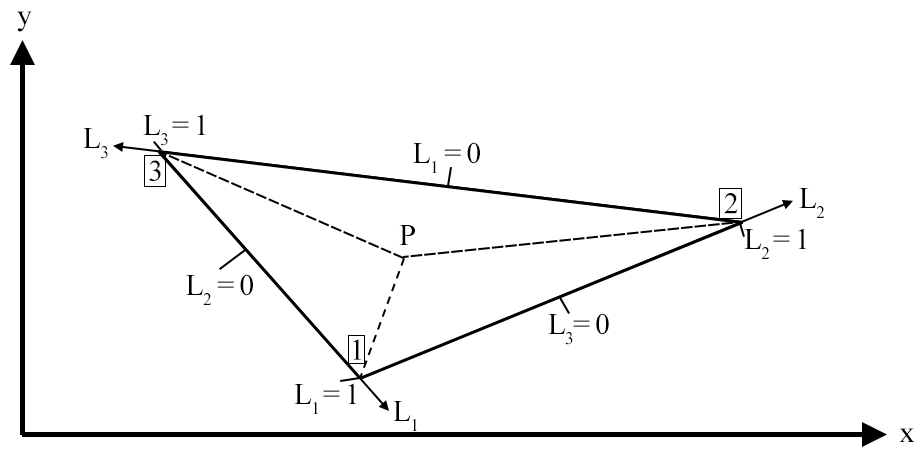
\includegraphics[width=0.9\linewidth]{figures/triangular_coords}
	\setlength\unitlength{0.9cm}
	\begin{picture}(14,6)
	\thicklines
	\put(0.4,0.3){\vector(1,0){13.5}}
	\put(0.4,0.3){\vector(0,1){5.5}}
	\put(14.0,0.2){$\mathbf{x}$}
	\put(0.3,5.9){$\mathbf{y}$}
	
	\put(6.2,0.7){\line(6,2.5){6}}
	\put(6.05,0.8){$1$}
	\put(12.2,3.2){\line(-10,1){10}}
	\put(12,3.3){$2$}
	\put(2.2,4.2){\line(4,-3.5){4}}
	\put(1.9,3.8){$3$}
	
	\thinlines
	\Dline(6.2,0.7)(6.5,2.5){0.1}
	\Dline(12.2,3.2)(6.5,2.5){0.1}
	\Dline(2.2,4.2)(6.5,2.5){0.1}
	\put(6.3,2.7){$P$}
	
	\put(12.2,3.2){\vector(6,2.5){0.5}}
	\put(12.8,3.3){$L_2$}
	\put(12.2,2.8){$L_2 = 1$}
	\put(6.2,0.7){\vector(4,-3.5){0.5}}
	\put(6.7,0.4){$L_1$}
	\put(4.9,0.4){$L_1 = 1$}
	\put(2.2,4.2){\vector(-10,1){0.7}}
	\put(1.0,4.2){$L_3$}
	\put(2.2,4.4){$L_3 = 1$}
	
	\put(9,1.5){$L_3 = 0$}
	\put(2.8,2.2){$L_2 = 0$}
	\put(7,4){$L_1 = 0$}
	\end{picture}
  	\caption{Triangular coordinates $L_1,L_2,L_3$ and sampling point $P$ within a triangular element. The nodes and edges represent special cases of triangular coordinates.}
  	\label{fig:tri_coords}
  \end{figure}
  
  % interpolationsbedingunen führen auf Formfunktionen\\
  To get the unknown coefficients $a_i$, values for the triangular coordinates are set. This creates a system of linear equations:
  \begin{align}
  \psi(L_1=1, L_2=0) = \psi_1 &\rightarrow \psi_1 = a_0 + a_1 \nonumber\\
  \psi(L_1=0, L_2=1) = \psi_2 &\rightarrow \psi_2 = a_0 + a_2 \nonumber\\
  \psi(L_1=0, L_2=0) = \psi_3 &\rightarrow \psi_3 = a_0
  \end{align}
  Written as matrix and vector:
  \begin{align}
  \underline{A} \vec{a} &= \vec{\psi} \nonumber\\
  \begin{pmatrix}
  1 & 1 & 0\\
  1 & 0 & 1\\
  1 & 0 & 0
  \end{pmatrix} \begin{pmatrix}
  a_0 \\ a_1 \\ a_2
  \end{pmatrix} &= \begin{pmatrix}
  \psi_1 \\ \psi_2 \\ \psi_3
  \end{pmatrix}
  \end{align}
  With the inverting of matrix $A$, the coefficients can be found:
  \begin{equation}\label{eq:t3_coeffsA}
  \vec{a} = \underline{A}^{-1} \vec{\psi} = \begin{pmatrix}
  0 & 0 & 1\\
  1 & 0 & -1\\
  0 & 1 & -1
  \end{pmatrix} \begin{pmatrix}
  \psi_1 \\ \psi_2 \\ \psi_3
  \end{pmatrix}
  \end{equation}
  If one puts equation \eqref{eq:t3_coeffsA} into \eqref{eq:t3_ansatz}, the shape functions for the three-node triangular finite element will be derived:
  \begin{align}\label{eq:t3SF}
  u &= \vec{x}^T \vec{a} = \vec{x}^T \underline{A}^{-1}\vec{u} = \vec{N}^T\vec{u} \nonumber\\
  \vec{N}^T &= \vec{x}^T \underline{A}^{-1} =
  \begin{pmatrix}
  1 & L_1 & L_2
  \end{pmatrix} \begin{pmatrix}
  0 & 0 & 1\\
  1 & 0 & -1\\
  0 & 1 & -1
  \end{pmatrix} \nonumber\\
  &= \begin{pmatrix}
  L_1 & L_2 & 1-L_1-L_2
  \end{pmatrix} = \begin{pmatrix}
  N_1 & N_2 & N_3
  \end{pmatrix}
  \end{align}
  Characteristically for a shape function $N_i$ is that it evaluates to 1 at node $i$ and to 0 at the two other nodes, as stated in~\cite{steinke2005finite}. The functions are linear with respect to $L_1$ and $L_2$ which can be seen in equation \eqref{eq:t3SF}. As stated before, these shape functions are the same for displacement $u$ and $v$. With the knowledge of the displacement values of the element's nodes, one can formulate the displacement functions in triangular coordinate notation as follows:
  \begin{align}
  u &= N_1 u_1 + N_2 u_2 + N_3 u_3 \nonumber\\
  v &= N_1 v_1 + N_2 v_2 + N_3 v_3
  \end{align}
  Or in matrix form:
  \begin{align} \label{eq:t3u=Nu}
  \vec{\tilde{u}} &= \underline{N} \vec{u} \nonumber\\
  \begin{pmatrix}
  u \\ v
  \end{pmatrix} &= \begin{pmatrix}
  N_1 & 0 & N_2 & 0 & N_3 & 0 \\
  0 & N_1 & 0 & N_2 & 0 & N_3
  \end{pmatrix} \begin{pmatrix}
  u_1 \\ v_1 \\ u_2 \\ v_2 \\ u_3 \\ v_3
  \end{pmatrix}
  \end{align}
  The vector $\vec{\tilde{u}}$ describes the element's displacements as product of matrix $\underline{N}$ containing the shape functions and vector $\vec{u}$ containing the displacements of the single triangle's nodes. Now, one can put equation \eqref{eq:t3u=Nu} into \eqref{eq:t3displ-str-rel}:
  \begin{equation}\label{eq:t3eps=Bu}
  \vec{\varepsilon} = \underline{L}\vec{\tilde{u}} = \underline{L}\;\underline{N} \vec{u} = \underline{B} \vec{u}
  \end{equation}
  The product of $\underline{L}$ and $\underline{N}$ is called \textit{strain-displacement matrix} $\underline{B}$.
  In order to calculate the strain-displacement matrix, one has to assemble the $\underline{L}$ matrix containing the first partial derivatives of the triangular element. With the chain rule applied, the partial derivatives look as follows:
  \begin{align}
  \frac{\partial}{\partial L_1} = \frac{\partial x}{\partial L_1} \frac{\partial}{\partial x} + \frac{\partial y}{\partial L_1} \frac{\partial}{\partial y} \nonumber\\
  \frac{\partial}{\partial L_2} = \frac{\partial x}{\partial L_2} \frac{\partial}{\partial x} + \frac{\partial y}{\partial L_2} \frac{\partial}{\partial y}
  \end{align}
  or shortened in matrix and vector notation:
  \begin{align}\label{eq:t3NablaTilde}
  \tilde{\nabla} &= \underline{J} \nabla \nonumber\\
  \begin{pmatrix}
  \frac{\partial}{\partial L_1}\\ \frac{\partial}{\partial L_2}
  \end{pmatrix} &= \begin{pmatrix}
  \frac{\partial x}{\partial L_1} & \frac{\partial y}{\partial L_1}\\
  \frac{\partial x}{\partial L_2} & \frac{\partial y}{\partial L_2}
  \end{pmatrix} \begin{pmatrix}
  \frac{\partial}{\partial x}\\ \frac{\partial}{\partial y}
  \end{pmatrix},
  \end{align}
  where $\underline{J}$ represents the Jacobian matrix, $\nabla$ the partial derivatives in Cartesian coordinates and $\tilde{\nabla}$ the partial derivatives in triangular coordinates. To get the derivatives in Cartesian form, the upper equation must be multiplied with the inverse Jacobian matrix $\underline{J}^{-1}$:
  \begin{equation}
  \underline{J}^{-1} = \frac{1}{|\underline{J}|} \begin{pmatrix}
  \frac{\partial y}{\partial L_2} & -\frac{\partial y}{\partial L_1} \\
  \frac{-\partial x}{\partial L_2} & \frac{\partial x}{\partial L_1}
  \end{pmatrix}
  \end{equation}
  where $|\underline{J}|$ denotes the determinant of the Jacobian matrix. The conversion between triangular and Cartesian coordinates can be summarized as follows (see Figure~\ref{fig:tri_coords} and~\cite{steinke2005finite}):
  \begin{align}\label{eq:triCoord<->CartCoord}
  L_1 &+ L_2 + L_3 = 1 \rightarrow L_3 = 1-L_1-L_2 \nonumber\\
  x &= x_1L_1 + x_2L_2 + x_3L_3 = (x_1-x_3)L_1 + (x_2-x_3)L2 + x_3\\
  y &= y_1L_1 + y_2L_2 + y_3L_3 = (y_1-y_3)L_1 + (y_2-y_3)L2 + y_3 \nonumber
  \end{align}
  Considering equation \eqref{eq:triCoord<->CartCoord} the Jacobian matrix can now be calculated:
  \begin{equation}
  J = \begin{pmatrix}
  \frac{\partial x}{\partial L_1} = x_1-x_3 = x_{13} & \frac{\partial y}{\partial L_1} = y_1-y_3 = y_{13}\\
  \frac{\partial x}{\partial L_2} = x_2-x_3 = x_{23} & \frac{\partial y}{\partial L_2} = y_2-y_3 = y_{23}
  \end{pmatrix} = \begin{pmatrix}
  x_{13} & y_{13}\\
  x_{23} & y_{23}
  \end{pmatrix}
  \end{equation}
  and hence the inverse Jacobian matrix:
  \begin{equation}\label{eq:t3invJac}
  \underline{J}^{-1} = \frac{1}{2 A_\triangle} \begin{pmatrix}
  y_{23} & -y_{13}\\
  -x_{23} & x_{13}
  \end{pmatrix}
  \end{equation}
  The determinant of the Jacobian matrix is two times the area of the triangle. With the help of equation \eqref{eq:t3invJac}, \eqref{eq:t3NablaTilde} can be reorganized:
  \begin{equation}\label{eq:nabla=invJ*nabla-tilde}
  \nabla = \underline{J}^{-1} \tilde{\nabla}
  \end{equation}
  and this finally yields the new version of the differential operator $\underline{L}$ \cite{steinke2005finite}:
  \begin{align}
  \underline{L} = \frac{1}{2 A_\triangle} \begin{pmatrix}
  y_{23}\frac{\partial}{\partial L_1} - y_{13}\frac{\partial}{\partial L_2} & 0 \\
  0 & -x_{23}\frac{\partial}{\partial L_1} + x_{13}\frac{\partial}{\partial L_2} \\
  -x_{23}\frac{\partial}{\partial L_1} + x_{13}\frac{\partial}{\partial L_2} & y_{23}\frac{\partial}{\partial L_1} - y_{13}\frac{\partial}{\partial L_2}
  \end{pmatrix}
  \end{align}
  
  % Dehnungs-Verschiebungs-Beziehung -> führt zu B + Spannungs-Verschiebungs-Beziehung\\
  Next, the strain-displacement matrix $\underline{B}$ can be calculated:
  \begin{align}
  \underline{B} &= \underline{L}\; \underline{N} \nonumber\\
  &= \frac{1}{2 A_\triangle} \begin{pmatrix}
  y_{23}\frac{\partial}{\partial L_1} - y_{13}\frac{\partial}{\partial L_2} & 0 \\
  0 & -x_{23}\frac{\partial}{\partial L_1} + x_{13}\frac{\partial}{\partial L_2} \\
  -x_{23}\frac{\partial}{\partial L_1} + x_{13}\frac{\partial}{\partial L_2} & y_{23}\frac{\partial}{\partial L_1} - y_{13}\frac{\partial}{\partial L_2}
  \end{pmatrix} \nonumber\\
  & \quad \begin{pmatrix}
  L_1 & 0 & L_2 & 0 & 1-L_1-L_2 & 0 \\
  0 & L_1 & 0 & L_2 & 0 & 1-L_1-L_2
  \end{pmatrix} \nonumber\\
  &= \frac{1}{2 A_\triangle} \begin{pmatrix}
  y_{23} & 0 & -y_{13} & 0 & y_{12} & 0 \\
  0 & -x_{23} & 0 & x_{13} & 0 & -x_{12} \\
  -x_{23} & y_{23} & x_{13} & -y_{13} & -x_{12} & y_{12}
  \end{pmatrix}
  \end{align}
  
  % Einsetzen in Gesamtpotential + Variation\\
  With $\underline{B}$ known, one can insert equation \eqref{eq:t3eps=Bu} into \eqref{eq:sigma=D*eps} to get the stresses:
  \begin{equation} \label{eq:t3sigma=DBu}
  \vec{\sigma} = \underline{D}\;\underline{B} \vec{u}
  \end{equation}
  Finally, every term of the plane element's functional \eqref{eq:planeFunctional} can be filled with the above discretized terms:
  \begin{align}\label{eq:t3functional}
  \Pi &= \frac{1}{2} \int_{V}\vec{\varepsilon}^T\vec{\sigma}\;dV - \vec{u}^T \vec{F} \nonumber\\
      &= \frac{1}{2} \int_{V}\vec{u}^T \underline{B}^T\underline{D}\;\underline{B}\vec{u}\;dV - \vec{u}^T \vec{F} \nonumber\\
      &= \frac{1}{2} \vec{u}^T \int_{V} \underline{B}^T\underline{D}\;\underline{B}\;dV \vec{u}- \vec{u}^T \vec{F} \nonumber\\
      &= \frac{1}{2}\vec{u}^T \underline{K} \vec{u} - \vec{u}^T \vec{F}
  \end{align}
  with $\underline{K}$ denoting the stiffness matrix and $\vec{F}$ the nodal force vector.
  
  % Bestimmung von K kürzen: wichtig ist nur s.221 K = t*int(H*dA,A) mit dV = t*dA
  The variation of the functional \eqref{eq:t3functional} is as follows~\cite{steinke2005finite}:
  \begin{align}
  \delta\Pi &= \frac{\partial\Pi}{\partial \vec{u}}\delta\vec{u} = 0 \nonumber\\
            &= \frac{1}{2}\delta\vec{u}^T\frac{\partial\vec{u}^T}{\partial\vec{u}^T}\underline{K}\vec{u} + \frac{1}{2}\vec{u}^T\underline{K}\frac{\partial\vec{u}}{\partial\vec{u}}\delta\vec{u} - \delta\vec{u}\frac{\partial\vec{u}^T}{\partial\vec{u}^T}\vec{F} \nonumber\\
            &= \delta\vec{u}^T\left(\underline{K}\vec{u}-\vec{F}\right) = 0
  \end{align}
  In order to satisfy this equation, the term in between the parenthesis must be zero ($\delta\vec{u}^T$ can have arbitrary values). This leads to the equilibrium equation of the triangular plane element as described in~\cite{steinke2005finite}:
  \begin{equation}
  \underline{K}\vec{u} = \vec{F}
  \end{equation}
  Since the thickness $t$ of the element is assumed to be constant, it holds $dV = t\ dA$ and therefore the integral of the stiffness matrix changes to:
  \begin{equation}
  \underline{K} = t \int_A \underline{B}^T\underline{D}\;\underline{B}\;dA = t A_\triangle \underline{B}^T\underline{D}\;\underline{B}
  \end{equation}
  
  
  
  \subsubsection{Quad-4 Plane Element}\label{sec:Shell-Plane-Quad}
  It is sometimes beneficial to use quadrilateral elements when describing certain detailed parts of a mesh or just to use less elements to describe a plane area. In contrast to triangles which always lie, due to their simple shape, in a plane, quadrilateral can have more complex forms. Such cases include for example: The fourth node does not lie in the plane defined by the other three or the shape is not convex. It is difficult to deal with such forms and one could be tempted to restrict the element to have rectangular shapes only, because these are easy to formulate and work with. But they are impractical when complicated geometry is to be modeled, especially if details should be emphasized in fine graduation.
    
  %- see Steinke~\cite{steinke2005finite} page 237-250 + Cook~\cite{cook2002concepts} page 202-208\\
  One solution to this problem is the use of isoparametric elements. They can be non-rectangular. The trick is to use reference coordinates which map the physical element into a reference element that is a square. Thus, the physical element can have a more general shape, but a coordinate transformation and numerical integration is needed which brings in more mathematical complexity~\cite{cook2002concepts}.
  
  In this section a quadrilateral isoparametric elements consisting of four nodes is described and denoted by \textbf{Quad-4}. Figure~\ref{fig:coord_trafo} shows the two abstraction layers: On the left side the original element is shown in physical space, on the right side the reference element is shown. The square has a side length of $2$. The coordinate system with the $\xi$ and $\eta$ axis has its origin in the center of the square. Also note the ordering of the nodes is counterclockwise.
  \begin{figure}[htbp]%- bild von original- und bildebene Bild 7.17 steinke oder 6.2-1. cook
  	\centering
  	%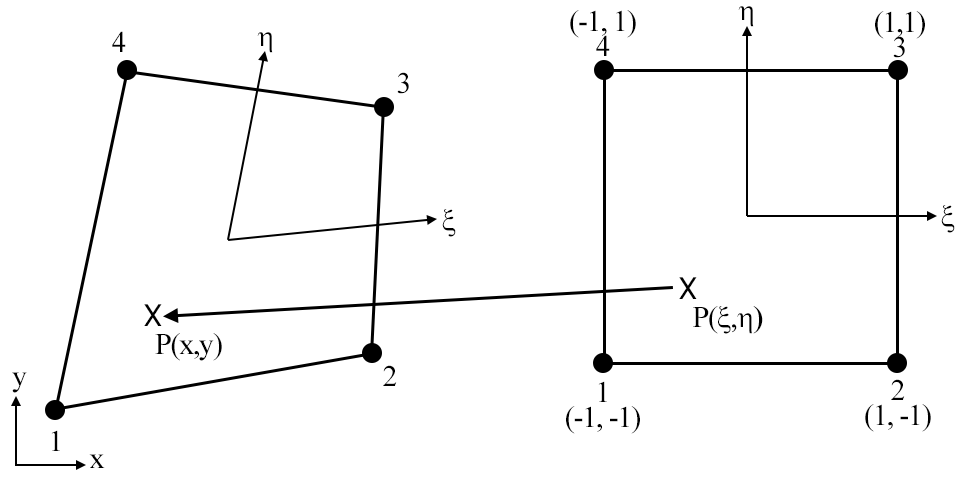
\includegraphics[width=0.97\linewidth]{figures/coord_trafo}
  	\setlength\unitlength{0.99cm}
  	\begin{picture}(14,6)
  	\thicklines
  	\put(0.4,0.3){\vector(1.5,0){1.5}}
  	\put(0.4,0.3){\vector(0,1.5){1.5}}
  	\put(2,0.2){$\mathbf{x}$}
  	\put(0.3,2){$\mathbf{y}$}
  	
  	\polyline(1,1)(6,2)(6.3,4.5)(2.5,5.3)(1,1)
  	\put(1,1){\circle*{0.2}}
  	\put(6,2){\circle*{0.2}}
  	\put(6.3,4.5){\circle*{0.2}}
  	\put(2.5,5.3){\circle*{0.2}}
  	\polyline(10,1)(13.5,1)(13.5,4.5)(10,4.5)(10,1)
  	\put(10,1){\circle*{0.2}}
  	\put(13.5,1){\circle*{0.2}}
  	\put(13.5,4.5){\circle*{0.2}}
  	\put(10,4.5){\circle*{0.2}}
  	
  	\thinlines
  	\put(11.75,2.75){\vector(2,0){2}}
  	\put(13.8,2.6){$\xi$}
  	\put(11.75,2.75){\vector(0,2){2}} 
  	\put(11.6,4.9){$\eta$}
  	
  	\put(3.95,3.2){\vector(2.7,0.2){2.7}}
  	\put(6.80,3.2){$\xi$}
  	\put(3.95,3.2){\vector(0.7,2.3){0.7}} 
  	\put(4.60,5.6){$\eta$}
  	
  	\put(9.6,0.8){$1$}
  	\put(9.3,0.5){$(-1,-1)$}
  	\put(13.7,0.8){$2$}
  	\put(12.7,0.5){$(1,-1)$}
  	\put(13.75,4.35){$3$}
  	\put(13.1,4.75){$(1,1)$}
  	\put(9.6,4.35){$4$}
  	\put(9.3,4.75){$(-1,1)$}
  	
  	\put(0.9,0.5){$1$}
  	\put(5.9,1.5){$2$}
  	\put(6.5,4.4){$3$}
  	\put(2.1,5.2){$4$}
  	
  	\put(10.75,1.75){$\times P(\xi,\eta)$}
  	\put(2.5,2.25){$\times$}
  	\put(2.3,1.9){$P(x,y)$}
  	\thicklines
  	\put(10.7,1.85){\vector(-7.9,0.55){7.9}}
  	\end{picture}
  	\caption{Coordinate transformation of four-node quadrilateral element with physical space on the left side and reference space on the right side}
  	\label{fig:coord_trafo}
  \end{figure}
  
  %- eigenschaften der ansatzfunktion + formfunktionen\\
  Similarly to the triangular element, interpolating the displacement field as well as the element geometry is done by shape functions. They are defined in reference coordinates. The displacement of a point within the element can be expressed by the displacements at the nodes and shape functions $\underline{N}$. Also, the position of that point can be expressed in terms of the (global) nodal positions and shape functions $\underline{\tilde{N}}$. The element is called \textit{isoparametric} if $\underline{N}$ is identical to $\underline{\tilde{N}}$. If $\underline{\tilde{N}}$ is of lower degree than $\underline{N}$, the element is called \textit{subparametric} and \textit{superparametric} if it is the other way around~\cite{cook2002concepts}.
  
  %- verschiebungen von uv mit formfunktionen und u darstellen\\
  Every node has two degrees of freedom: A displacement $u$ along the x-axis and a displacement $v$ along the y-axis. To find the shape functions it does not matter which variable to choose, so the following test function was used for $\phi$ representing $u$ or $v$~\cite{steinke2005finite}:
  \begin{equation}\label{eq:q4basis}
  \phi(\xi,\eta) = a_0 + a_1\xi + a_2\eta + a_3\xi\eta = \begin{pmatrix}
  1&\xi&\eta&\xi\eta
  \end{pmatrix}\begin{pmatrix}
  a_0\\a_1\\a_2\\a_3
  \end{pmatrix} = \vec{x}^T\vec{a}
  \end{equation}
  The interpolation conditions at the nodes are as follows:
  \begin{align}
  \phi(-1,-1) &= \phi_1 \rightarrow \phi_1 = a_0 -a_1 -a_2 +a_3 \nonumber\\
  \phi(1,-1) &= \phi_2 \rightarrow \phi_2 = a_0 +a_1 -a_2 -a_3 \nonumber\\
  \phi(1,1) &= \phi_3 \rightarrow \phi_3 = a_0 +a_1 +a_2 +a_3 \nonumber\\
  \phi(-1,1) &= \phi_4 \rightarrow \phi_4 = a_0 -a_1 +a_2 -a_3
  \end{align}
  or in matrix-vector notation:
  \begin{align}
  \underline{A}\vec{a} &= \vec{\phi} \nonumber\\
  \begin{pmatrix}
  1 &-1&-1& 1\\
  1 & 1&-1&-1\\
  1 & 1& 1& 1\\
  1 &-1& 1&-1
  \end{pmatrix} \begin{pmatrix}
  a_0\\a_1\\a_2\\a_3
  \end{pmatrix} &= \begin{pmatrix}
  \phi_1\\\phi_2\\\phi_3\\\phi_4
  \end{pmatrix}
  \end{align}
  Inversion of $\underline{A}$ yields the coefficients $a_i$ of $\vec{a}$:
  \begin{equation}
  \vec{a} = \underline{A}^{-1}\vec{\phi} = \frac{1}{4} \begin{pmatrix}
  1&1&1&1\\
  -1&1&1&-1\\
  -1&-1&1&1\\
  1&-1&1&-1
  \end{pmatrix} \begin{pmatrix}
  \phi_1\\\phi_2\\\phi_3\\\phi_4
  \end{pmatrix}
  \end{equation}
  Inserting the last equation into \eqref{eq:q4basis}, one gets the shape functions $\vec{N}$ for the quadrilateral element:
  \begin{align}
  \phi &= \vec{x}^T\underline{A}^{-1}\vec{\phi} \nonumber\\
    &= \vec{N}^T\vec{\phi} \nonumber\\
    &= \frac{1}{4} \begin{pmatrix}
    1&\xi&\eta&\xi\eta
    \end{pmatrix} \begin{pmatrix}
    1&1&1&1\\
    -1&1&1&-1\\
    -1&-1&1&1\\
    1&-1&1&-1
    \end{pmatrix} \vec{\phi} \nonumber\\
    &= \begin{pmatrix}
    \frac{1}{4}(1-\xi)(1-\eta)&\frac{1}{4}(1+\xi)(1-\eta)&\frac{1}{4}(1+\xi)(1+\eta)&\frac{1}{4}(1-\xi)(1+\eta)
    \end{pmatrix} \vec{\phi}
  \end{align}
  One can evaluate shape function $i$ with the $\xi\eta$-coordinates of node $i$. If it evaluates to 1 while at any other node coordinates it evaluates to zero, the shape function is correctly set. Now, the displacements can be expressed as follows:
  \begin{equation}
  \vec{\tilde{u}} = \begin{pmatrix}
  u\\v
  \end{pmatrix} = \underline{N}\vec{u} = \begin{pmatrix}
  N_1&0&N_2&0&N_3&0&N_4&0\\
  0&N_1&0&N_2&0&N_3&0&N_4
  \end{pmatrix} \begin{pmatrix}
  u_1\\v_1\\u_2\\v_2\\u_3\\v_3\\u_4\\v_4
  \end{pmatrix}
  \end{equation}
  with $\underline{N}$ being the matrix containing the shape functions and $\vec{u}$ being the vector of the nodal displacements.
  
  %- jacobi-matrix aufstellen, inverse und determinante nicht so genau (bzw. einfach, weil J eh nur 2x2 ist)\\
  The assembly of the strain-displacement matrix $\underline{B}$ is more complicated with isoparametric elements. Due to the $\xi\eta$-coordinates one cannot easily describe an operator such as $\partial/\partial x$. The first step is to formulate a function $\phi = \phi(\xi,\eta)$. Like in the derivation on the shape functions $\phi$ can represent $u$ or $v$. Derivatives with respect to $\xi$ and $\eta$ are as follows~\cite{cook2002concepts}:
  \begin{align}
  \frac{\partial \phi}{\partial \xi} = \frac{\partial \phi}{\partial x} \frac{\partial x}{\partial \xi} + \frac{\partial \phi}{\partial y} \frac{\partial y}{\partial \xi} \nonumber\\
  \frac{\partial \phi}{\partial \eta} = \frac{\partial \phi}{\partial x} \frac{\partial x}{\partial \eta} + \frac{\partial \phi}{\partial y} \frac{\partial y}{\partial \eta}
  \end{align}
  or in matrix notation:
  \begin{equation}\label{eq:q4derivRS=J*derivXY}
  \vec{\tilde{\phi}} = \underline{J} \vec{\phi}
  \end{equation}
  where $\underline{J}$ is the Jacobian matrix
  \begin{equation}
  \underline{J} = \begin{pmatrix}
  \sum N_{i,\xi}x_i & \sum N_{i,\xi}y_i\\
  \sum N_{i,\eta}x_i & \sum N_{i,\eta}y_i
  \end{pmatrix}
  \end{equation}
  and $N_{i,j}$ denotes the derivation of the $i$-th shape function with respect to $j$. $x_i$ is the $i$-th component of the $\vec{x}$-vector. The Jacobian matrix can be written out as follows:
  \begin{align}
  \underline{J} &= \frac{1}{4}\begin{pmatrix}
  -(1-\eta) & (1-\eta) & (1+\eta) & -(1+\eta)\\
  -(1-\xi) & -(1+\xi) & (1+\xi) & (1-\xi)
  \end{pmatrix} \begin{pmatrix}
  x_1 & y_1\\
  x_2 & y_2\\
  x_3 & y_3\\
  x_4 & y_4
  \end{pmatrix} \nonumber\\
  &= \begin{pmatrix}
  (x_{12}+x_{34})\eta - x_{12} + x_{34} & (y_{12} + y_{34})\eta - x_{12} + y_{34}\\
  (x_{12}+x_{34})\xi  - x_{13} - x_{24} & (y_{12} + y_{34})\xi  - y_{13} + y_{24}
  \end{pmatrix}
  \end{align}
  Next, equation \eqref{eq:q4derivRS=J*derivXY} can be rearranged to get the derivatives with respect to $x$ and $y$:
  \begin{equation}
  \vec{\phi} = \underline{J}^{-1}\vec{\tilde{\phi}}
  \end{equation}
  
  %- dehnungs-verschiebungs-beziehung
  \noindent With the derivatives calculated, the strain-displacement relation \eqref{eq:displ_strain_relation} can be obtained \cite{cook2002concepts}:
  \begin{align}
  \vec{\varepsilon} &= \begin{pmatrix}
  \frac{\partial u}{\partial x} \\
  \frac{\partial v}{\partial y} \\
  \frac{\partial u}{\partial y} + \frac{\partial v}{\partial x}
  \end{pmatrix} = \underbrace{\begin{pmatrix}
  1&0&0&0\\
  0&0&0&1\\
  0&1&1&0
  \end{pmatrix}} \begin{pmatrix}
  {\partial u}/{\partial x} \\ {\partial u}/{\partial y} \\ {\partial v}/{\partial x} \\ {\partial v}/{\partial y}
  \end{pmatrix} \\
  &\qquad\qquad\qquad\qquad\qquad\,\: \underline{L} \nonumber
  \end{align}
  \begin{align}
  \begin{pmatrix}
  {\partial u}/{\partial x} \\ {\partial u}/{\partial y} \\ {\partial v}/{\partial x} \\ {\partial v}/{\partial y}
  \end{pmatrix} &= \underbrace{\begin{pmatrix}
  j_{11} & j_{12} & 0 & 0\\
  j_{21} & j_{22} & 0 & 0\\
  0 & 0 & j_{11} & j_{12}\\
  0 & 0 & j_{21} & j_{22}
  \end{pmatrix}} \begin{pmatrix}
  {\partial u}/{\partial \xi} \\ {\partial u}/{\partial \eta} \\ {\partial v}/{\partial \xi} \\ {\partial v}/{\partial \eta}
  \end{pmatrix}\\
  &\qquad\qquad\quad\,\: \underline{\hat{J}} \nonumber
  \end{align}
  \begin{align}
  \begin{pmatrix}
  {\partial u}/{\partial \xi} \\ {\partial u}/{\partial \eta} \\ {\partial v}/{\partial \xi} \\ {\partial v}/{\partial \eta}
  \end{pmatrix} &= \underbrace{\begin{pmatrix}
  N_{1,\xi}  & 0 N_{2,\xi}  & 0 & N_{3,\xi}  & 0 & N_{4,\xi}  & 0\\
  N_{1,\eta} & 0 N_{2,\eta} & 0 & N_{3,\eta} & 0 & N_{4,\eta} & 0\\
  0 & N_{1,\xi}  & 0 N_{2,\xi}  & 0 & N_{3,\xi}  & 0 & N_{4,\xi}\\
  0 & N_{1,\eta} & 0 N_{2,\eta} & 0 & N_{3,\eta} & 0 & N_{4,\eta}
  \end{pmatrix}} \begin{pmatrix}
  u_1\\v_1\\u_2\\v_2\\u_3\\v_3\\u_4\\v_4
  \end{pmatrix}\\
  &\qquad\qquad\qquad\qquad\qquad\quad\; \underline{\hat{N}} \nonumber
  \end{align}
  where $j_{i}$ denotes the $i$-th entry of the inverse Jacobian matrix.
  The composition of the previous three equations forms the matrix $\underline{B}$:
  \begin{equation}
  \underline{B} = \underline{L}\,\underline{\hat{J}}\,\underline{\hat{N}}
  \end{equation}
  

  %- stefigkeitsmatrix $K = int_V(B^TDBdV) = t*int_V(B^TDBdA) = t*int_-1^1 int_-1^1(B^TDB|J|dsdr)$ + erwähnen, dass |J| Flächeninhalt angibt (ref finden)
  Together with the functional equation \eqref{eq:t3functional} and the material matrix $\underline{D}$ (eq. \eqref{eq:sigma=D*eps}), the stiffness matrix for the quadrilateral isoparametric element can be written as:
  \begin{equation}
  \underline{K} = \int_V \underline{B}^T \underline{D}\,\underline{B}\, dV = t\int_A \underline{B}^T \underline{D}\,\underline{B}\, dA = t\int_{-1}^{1}\int_{-1}^{1} \underline{B}^T \underline{D}\,\underline{B}\, |\underline{J}| d\xi d\eta
  \end{equation}
  For the Quad-4 element, a Gaussian quadrature needs four Gauss integration points to satisfy the above equation~\cite{steinke2005finite}. These four points are located at $\xi_i = \pm \frac{\sqrt{3}}{3}$ and $\eta_i = \pm \frac{\sqrt{3}}{3}$ with weight factors $\omega_i = 1$. The equation for the stiffness matrix can then be written in discretized form as follows:
  \begin{equation}
  \underline{K} = t \sum_{i=1}^{2} \sum_{j=1}^{2} \omega_i \omega_j \underline{B}(\xi_i,\eta_j)^T \underline{D}\, \underline{B}(\xi_i,\eta_j) |\underline{J}(\xi_i,\eta_j)|
  \end{equation}
 
 \subsection{Plate Bending Element}\label{sec:Shell-Plate}
  In contrast to the plane element, the loads at the plate elements are applied transversal to the element's mid-surface producing plate bending. It has one deformation degree of freedom and two rotational degrees of freedom. Plate elements are often used to model floors or ceilings. In this section, the plate element is discussed in more detail and two discretizations are described: The three-node triangular plate element and the four-node quadrilateral plate element.  
  
  \subsubsection{Problem Definition}\label{sec:Shell-Plate-ProbDef}
  %\cite{steinke2005finite} ch8.1
  \begin{figure}[htbp] % bild wie bei~\ref{sec:MprobDef}
  	\centering
  	%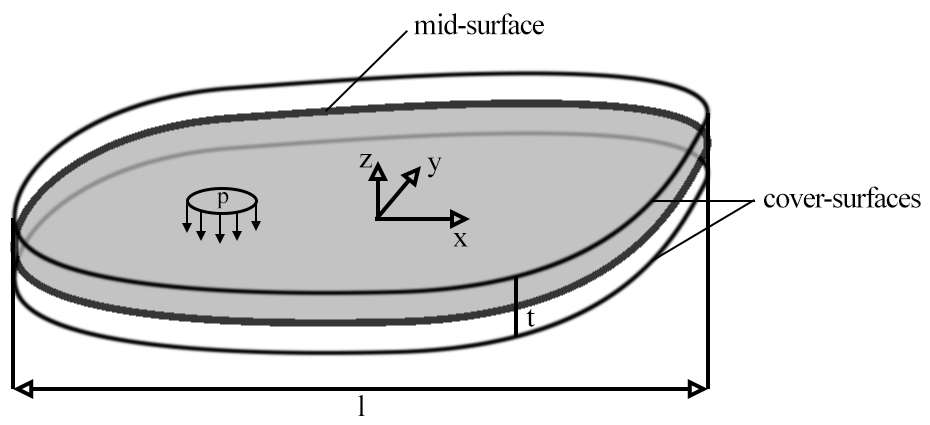
\includegraphics[width=0.9\linewidth]{figures/plate}
  	\setlength\unitlength{1.0cm}
  	\begin{picture}(12,6)
  	\thinlines
  	\put(0,0){\pgfsetfillopacity{1.0}\Curve(0.5,2.5)<0,0.25>(3.5,4.25)<1,0.125>(7.5,4.5)<1,0>(10,2.5)<-1,-1>(6,1)<-0.5,-0.05>(2.5,1)<-0.5,0.125>(0.5,2.5)<0,0.5>}
  	\thicklines
  	{\pgfsetfillopacity{0.8}\color{gray}\Curve*(0.5,3)<0,0.25>(3.5,4.75)<1,0.125>(7.5,5)<1,0>(10,3)<-1,-1>(6,1.5)<-0.5,-0.05>(2.5,1.5)<-0.5,0.125>(0.5,3)<0,0.5>}
  	\put(0,0){\pgfsetfillopacity{1.0}\color{black}\Curve(0.5,3)<0,0.25>(3.5,4.75)<1,0.125>(7.5,5)<1,0>(10,3)<-1,-1>(6,1.5)<-0.5,-0.05>(2.5,1.5)<-0.5,0.125>(0.5,3)<0,0.5>}
    \put(6.6,2.9){$x$}
    \put(5.5,3){\vector(1,0){1}}
    \put(6.1,3.4){$y$}
    \put(5.5,3){\vector(0.5,0.65){0.5}}
    \put(5.4,4.1){$z$}
    \put(5.5,3){\vector(0,1){1}}
  	\thinlines
  	\put(0,0){\pgfsetfillopacity{1.0}\Curve(0.5,3.5)<0,0.25>(3.5,5.25)<1,0.125>(7.5,5.5)<1,0>(10,3.5)<-1,-1>(6,2)<-0.5,-0.05>(2.5,2)<-0.5,0.125>(0.5,3.5)<0,0.5>}
  	\Dline(0.5,3.5)(0.5,0.5){0.1}
  	\Dline(10.37,3.5)(10.37,0.5){0.1}
  	\put(5,0.5){\vector(-4.5,0){4.5}}
  	\put(5,0.5){\vector(5.37,0){5.37}}
  	\put(5.4,0.15){$l$}
  	\Line(2.5,2)(2.5,1)\put(2.43,0.7){$t$}
  	\polyline(10,3.5)(11,3)(10,2.5)\put(11.1,2.9){cover-surfaces}
  	\Line(7.5,5)(9.5,5.5)\put(9.6,5.4){mid-surface}
  	
  	\put(2.5,3){\cbezier(0,0)(0,0.25)(1,0.25)(1,0)}\put(2.5,3){\cbezier(0,0)(0,-0.25)(1,-0.25)(1,0)}\put(2.9,2.9){$p$}
  	\put(2.5,3.5){\vector(0,-0.5){0.5}}\put(3.5,3.5){\vector(0,-0.5){0.5}}\put(3,3.67){\vector(0,-0.5){0.5}}
  	\end{picture}
  	\caption{Schematic drawing of a Kirchhoff plate with its main dimension $l$, thickness $t$ and loading $p$ normal to the mid-surface}
  	\label{fig:plate}
  \end{figure}
  In contrast to a plane, where the load is located planar with respect to the mid-surface, the load is perpendicular to the mid-surface at a plate. Therefore plate element problems are important for supporting structures of bridges or ceilings and floors in buildings, for instance. In Figure~\ref{fig:plate} one can see a generalized plate object. It has a main dimension of $l$ and a constant thickness $t$. With the assumption that $t \ll l$, the problem becomes two dimensional and, instead of the whole object, only the middle plane between the two surface areas will be considered. The object has a local coordinate system with its xy-plane the mid-surface and its z-axis perpendicular to this plane. The cover-surfaces are located at $z = \pm t/2$. As stated in the beginning, the load is applied in z-direction, i.e. normal to the mid-surface.
  
  % hier wird die kirchhoff-platten-theorie verwendet
  In this work Kirchhoff's theory of thin plates is used. For thick plates or laminated plates, the theory of Reissner-Mindlin is more applicable~\cite{werkle1995finite}. The main difference is that with Reissner-Mindlin plates one takes the shear deformations into account. Thus, the normal to the mid-surface remains straight but not necessarily perpendicular to it; instead of a Kirchhoff plate: Here, the normal remains normal to the mid-surface even after deformation.
  
  % voraussetzungen der kirchhoff-platte
  The following conditions must be satisfied for a Kirchhoff plate~\cite{steinke2005finite}:
  \begin{itemize}
  	\item The thickness $t$ must be much smaller than the main dimension $l$: $t \ll l$.
  	\item Straight lines normal to the mid-surface remain straight after deformation.
  	\item Straight lines normal to the mid-surface remain normal to the mid-surface after deformation.
  	\item There is only a small amount of deformation $w$, i.e. $w < t$ and it holds $w \ne w(z)$.
  	\item The plate is symmetrical to the mid-surface and changes in thickness must be very small.
  	\item Normal stresses in z-direction $\sigma_{zz}$ will be neglected.
  \end{itemize}
  
  % größen der platte: durchbiegung w + verdrehungen dw/dx bzw. dw/dy
  With~\cite{klein2013fem} and~\cite{steinke2005finite} the following displacement terms can be formulated:
  \begin{align}
  w &= w(x,y) \\
  u &= -z \frac{\partial w}{\partial x}\\
  v &= -z \frac{\partial w}{\partial y}
  \end{align}
  The deformation $w$ suffices to explain the whole displacement vector. The two derivatives in the equations above describe the torsions around the x- and y-axis.

  % dehnungs-verschiebungs-beziehung
  Similar to the plane element, the Kirchhoff plate element can be in plane strain or plane stress, respectively~\cite{steinke2005finite}, i.e. equation \eqref{eq:displ_strain_relation} can be applied here, too:
  \begin{align}
  \vec{\hat{u}} &= \begin{pmatrix}
  u\\v
  \end{pmatrix} = -z \begin{pmatrix}
  \frac{\partial w}{\partial x}\\ \frac{\partial w}{\partial y}
  \end{pmatrix} = -z \nabla w \nonumber\\
  \vec{\varepsilon} &= \underline{L} \vec{\hat{u}} = -z \underline{L} \nabla w = -z \vec{\Delta} w = -z \vec{\kappa} \label{eq:eps=-z*kappa}\\
  \vec{\Delta} &= \underline{L} \nabla = \begin{pmatrix}
  \frac{\partial}{\partial x} & 0\\
  0 & \frac{\partial}{\partial y}\\
  \frac{\partial}{\partial y} & \frac{\partial}{\partial x}
  \end{pmatrix} \begin{pmatrix}
  \frac{\partial}{\partial x} & \frac{\partial}{\partial y}
  \end{pmatrix} = \begin{pmatrix}
  \frac{\partial^2}{\partial x^2}\\
  \frac{\partial^2}{\partial y^2}\\
  2\frac{\partial^2}{\partial x\partial y}
  \end{pmatrix} \nonumber\\
  \vec{\kappa} &= \vec{\Delta}w = \begin{pmatrix}
  \frac{\partial^2w}{\partial x^2}\\
  \frac{\partial^2w}{\partial y^2}\\
  2\frac{\partial^2w}{\partial x\partial y}
  \end{pmatrix} \label{eq:kappa=Delta*w}
  \end{align}
  
  % stoffgleichung (krümmungs-momenten-beziehung) -> führt auf Dp und Querkräfte Qx,Qy
  Referring~\cite{klein2013fem} ($\sigma_{zz} = 0, \tau_{xz} = \tau_{yz} = 0$), equation \eqref{eq:stress-strain-relation} can be filled with the above information:
  \begin{align}\label{eq:sigma=-z*D*kappa}
  \vec{\sigma} &= \underline{D} \vec{\varepsilon} = -z \underline{D} \vec{\kappa} \nonumber\\
               &= -\frac{E z}{1-\nu^2} \begin{pmatrix}
               1&\nu&0\\
               \nu&1&0\\
               0&0&\frac{1-\nu}{2}
               \end{pmatrix} \begin{pmatrix}
               \kappa_x\\\kappa_y\\2\kappa_{xy}
               \end{pmatrix}
  \end{align}
  The integration of the stresses $\vec{\sigma}$ over the thickness results in the vector of moments $\vec{M}^T = \left(M_{xx}\ \;M_{yy}\ \;M_{xy}\right)$~\cite{steinke2005finite}:
  \begin{equation}\label{eq:M=-Dp*kappa}
  \vec{M} = \int_{-t/2}^{t/2} z\vec{\sigma} dz = -\int_{-t/2}^{t/2} z^2 \underline{D} \vec{\kappa} dz = -\underline{D} \vec{\kappa} \int_{-t/2}^{t/2} z^2 dz = -\frac{t^3}{12} \underline{D} \vec{\kappa} = -\underline{D}_p \vec{\kappa}
  \end{equation}
  The above equation relates the moments with the curvatures of the plate. The integrals over the transverse stresses $\sigma_{xz}$ and $\sigma_{yz}$ lead to the following shear forces, as described in~\cite{steinke2005finite}:
  \begin{align}
  Q_x &= \int_{-t/2}^{t/2}\sigma_{xz} dz = \int_{-t/2}^{t/2} \sigma_{xz}^{\max} \left(1-4\left(\frac{z}{t}\right)^2\right)dz = \frac{2}{3} \sigma_{xz}^{\max} t \nonumber\\
  &= \frac{2}{3} \sigma_{xz}(z=0) t
  \end{align}
  \begin{align}
  Q_y &= \int_{-t/2}^{t/2}\sigma_{yz} dz = \int_{-t/2}^{t/2} \sigma_{yz}^{\max} \left(1-4\left(\frac{z}{t}\right)^2\right)dz = \frac{2}{3} \sigma_{yz}^{\max} t \nonumber\\
  &= \frac{2}{3} \sigma_{yz}(z=0) t
  \end{align}
  The transverse stress is distributed quadratically over the thickness t, i.e. they have their maximum at $z=0$ and vanish at $z = \pm \frac{t}{2}$. The equilibrium of forces in z-direction leads to:
  \begin{equation}\label{eq:dQx+dQy+p=0}
  \frac{\partial Q_x}{\partial x} + \frac{\partial Q_y}{\partial y} + p = 0
  \end{equation}
  with $p$ being the load applied perpendicular to the mid-surface. Additionally the equilibrium of moments around the x- and y-axis:\\
  \begin{align}\label{eq:dMxx+dMxy+Qx=0}
  \frac{\partial M_{xx}}{\partial x} + \frac{\partial M_{xy}}{\partial y} + Q_x &= 0 \nonumber\\
  \frac{\partial M_{yy}}{\partial y} + \frac{\partial M_{xy}}{\partial x} + Q_y &= 0
  \end{align}
  % gleichgewichtsbeziehung der platte (p ist flächenlast; näher untersuchen)
  Putting equation \eqref{eq:dMxx+dMxy+Qx=0} into \eqref{eq:dQx+dQy+p=0} results in:
  \begin{equation}\label{eq:Delta^T*M=p}
  \frac{\partial^2 M_{xx}}{\partial x^2} + \frac{\partial^2 M_{yy}}{\partial y^2} + 2\frac{\partial^2 M_{xy}}{\partial x\partial y} = \vec{\Delta}^T \vec{M} = p
  \end{equation}
  Now, one can insert the kinematic equation \eqref{eq:kappa=Delta*w} into equation \eqref{eq:M=-Dp*kappa} and then into the equilibrium relation \eqref{eq:Delta^T*M=p}:
  \begin{align}
  \vec{\kappa} &= \vec{\Delta}w \nonumber\\
  \vec{M} &= -\underline{D}_p \vec{\kappa} = -\underline{D}_p \vec{\Delta} w \nonumber\\
  \vec{\Delta}^T \vec{M} &= -\vec{\Delta}^T \underline{D}_p \vec{\Delta} w = p
  \end{align}
  The last equation leads to the partial differential equation of the plate bending~\cite{klein2013fem}:
  \begin{equation}
  \frac{\partial^4 w}{\partial x^4} + \frac{\partial^4 w}{\partial y^4} + 2\frac{\partial^4 w}{\partial x^2 \partial y^2} = -\frac{12(1-\nu^2)}{E t^3} p = \frac{p}{k}
  \end{equation}
  with $k$ denoted as \textit{plate stiffness}.
  
  % auf verschiedene randbedingungen der platte eingehen
  \begin{figure}[htbp] % Bild 8.5 steinke
  	\centering
  	%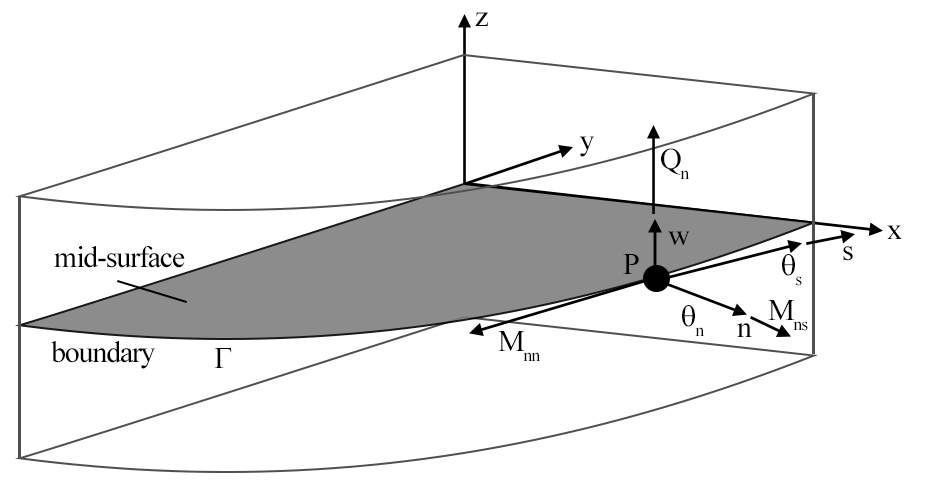
\includegraphics[width=0.97\linewidth]{figures/plate_boundary}
  	\setlength\unitlength{1.0cm}
  	\begin{picture}(13,5.5)
  	\thicklines
  	\put(12.8,3.1){$x$}
  	\put(0,2){\vector(7,1.5){8.5}}
  	\put(8.6,3.8){$y$}
  	\put(7,3.5){\vector(0,2){2}}
  	\put(7.2,5.4){$z$}
  	\put(7,3.5){\vector(5,-0.5){6}}
  	\thinlines
  	\polyline(0,0.5)(0,3.5)(7,5)(12,4.5)(12,1.5)
  	\Dline(7,2)(7,3.5){0.1}
  	\Dline(7,2)(0,0.5){0.1}
  	\Dline(7,2)(12,1.5){0.1}
  	{\pgfsetfillopacity{0.8}\color{gray}\Curve*(0,2)<1,-0.1>(12,3)<7,3>(12,3)<0,0>(7,3.5)<0,0>(0,2)<0,0>}
  	\put(0,0){\pgfsetfillopacity{1.0}\Curve(0,2)<1,-0.1>(12,3)<7,3>}
  	\put(0,0.5){\cbezier(0,0)(1,-0.1)(7,-1)(12,1)}
  	\put(0,3.5){\cbezier(0,0)(1,-0.1)(7,-1)(12,1)}
  	\thicklines
  	\put(10,2.31){\circle*{0.2}}\put(9.65,2.35){$P$}
  	\put(10,2.31){\vector(0,1){1.3}}\put(10.1,2.8){$w$}
  	\put(10,3.66){\vector(0,1){0.7}}\put(10.1,3.65){$Q_n$}
  	\put(10,2.31){\vector(1,0.25){1.5}}\put(11.1,2.25){$\theta_s$}
  	\put(11.6,2.7){\vector(1,0.25){0.75}}\put(12.1,2.55){$s$}
  	\put(10,2.31){\vector(-1,-0.25){1.5}}\put(8.75,1.7){$M_{nn}$}
  	\put(10,2.31){\vector(1,-0.4){1}}\put(10.4,1.75){$n$}
  	\put(11.1,1.85){\vector(1,-0.4){0.5}}\put(11.1,1.45){$\theta_n$}\put(11.3,1.85){$M_{ns}$}
  	\Line(1.4,2.7)(2.3,2.1)\put(0.5,2.8){mid-surface}
  	\put(0.5,1.4){boundary}
  	\put(3,1.35){$\Gamma$}
  	\end{picture}
  	\caption{Part of a plate's boundary with its essential and natural boundary conditions}
  	\label{fig:plate_boundary}
  \end{figure}
  Let $P$ be a point on the continuous boundary of the plate with a local Cartesian coordinate system as described in~\cite{steinke2005finite} (see Figure~\ref{fig:plate_boundary}): The $n$ coordinate is perpendicular to the boundary surface, the $s$ axis tangential to it. The third axis equals the global z-axis of the plate. There are three essential and three natural boundary conditions defined for $P$: The displacement $w$, the twists $\theta_n = \partial w/\partial s, \theta_s = -\partial w/\partial n$, the shear force $Q_n$ and the moments $M_{ns}$ and $M_{nn}$. Since this leads to an inconsistency with the differential equation above,~\cite{steinke2005finite} stated that Kirchhoff introduced new forces:
  \begin{equation}
  V_n = Q_n - \frac{\partial M_{ns}}{\partial s}
  \end{equation}
  With them, only the four conditions for $w, \theta_s, V_n$ and $M_{nn}$ occur.
  The plate can be mounted in different ways:
  \begin{itemize}
  	\item clamped: $w = 0, \theta_s = -\partial w/\partial n = 0$
  	\item simple supported: $w = 0, M_{nn} = 0$
  	\item symmetrical edge: $\theta_s = -\partial w/\partial n = 0, V_n = 0$
  \end{itemize}

  % funktional der platte
  The plate's functional as described in~\cite{steinke2005finite} is given below:
  \begin{equation}
  \frac{1}{2} \int_V \vec{\varepsilon}^T \vec{\sigma}\, d\:\!V
  \end{equation}
  One can insert equation \eqref{eq:eps=-z*kappa} and \eqref{eq:sigma=-z*D*kappa} into the functional:
  \begin{equation}
  \frac{1}{2} \int_V \vec{\varepsilon}^T \vec{\sigma}\, d\:\!V = \frac{1}{2}\int_V \vec{\kappa}^T \underline{D} \vec{\kappa} z^2\, d\!V = \frac{1}{2} \int_A \vec{\kappa}^T \underline{D}_p \vec{\kappa}\, d\!A
  \end{equation}
  Together with the potential of the external forces, the overall potential of the Kirchhoff plate is:
  \begin{equation}\label{eq:plateFunctional}
  \Pi = \frac{1}{2}\int_A \vec{\kappa}^T \underline{D}_p \vec{\kappa}\, dA
  - \int_A p\ w\, d\!A
  - \int_{\Gamma}\left(V_n w - M_{nn} \theta_s\right)\,d\:\!\Gamma
  \end{equation}
  
  % forderungen an plattenelement
  Klein~\cite{klein2013fem} states that for the plate element discretization additional conditions must be satisfied. They are: The bending $w(x,y)$ as well as the normal derivative $\partial w/\partial n$ at the element's boundary must be continuous to the neighboring elements. This would be the case if the bending and the normal derivative are explicitly determined by the nodal parameters at the border. Further,~\cite{klein2013fem} lists requirements for a plate element approach:
  \begin{itemize}
  	\item Totality of the displacement approach in order to guarantee good convergence.
  	\item The terms $1, x, y, x^2, xy, y^2$ should be included to get variable strains, curvatures and rigid body motion.
  \end{itemize}
  Steinke~\cite{steinke2005finite} expands the requirements as follows:
  \begin{itemize}
  	\item Compatibility of the displacement variable at the element's boundary (conformity condition): If the steadiness of the deformation $w$ and its first derivatives is not satisfied the bending surface between two elements can have a sharp bend at which the elements are overlapping at one side and diverge on the opposite side. If such a behavior is shown, the element is called \textit{non-conforming}.
  	\item Rigid body motions must not create strains and stresses in the element. This requires a constant term in the test function for the translative part of the motion and a linear term for the rotatory.
  	\item The test function must provide constant plain strain and plain stress: If the element converges in its size until it becomes a point, a constant state of bending must be describable in this situation. Since the bending is described as second order derivatives of $w$, the test function must include quadratic terms.
  \end{itemize}
  The following sections show details of two discretizations of plate elements: A triangular element with three nodes and a quadrilateral element with four nodes.
  
  \subsubsection{Tri-3 Plate Element}\label{sec:Shell-Plate-Tri}
  There exist many different types of triangular plate elements, introduced for example in~\cite{batoz1980study}, \cite{tocher1963analysis} and~\cite{specht1988modified}. The three-node triangular element from~\cite{tocher1963analysis} has three degrees of freedom (d.o.f) ($w, \theta_x, \theta_y$) per node. Its test function is a complete cubic polynomial. The term $xy$ was left out, because the polynomial has one coefficient more than the element has d.o.f. This leads to the problem that no constant state of bending can be described (non-conforming element) and this leads to wrong results at convergence~\cite{steinke2005finite}. Therefore,~\cite{steinke2005finite} challenges the practical use of this element. A possible way to use a complete cubic polynomial would be to add another node in the triangle's center of mass and assign $w$ as the only d.o.f to it~\cite{steinke2005finite}. But the problem of non-conformity persists, as the nodal twists don't suffice to describe the twists along the element's edges, which are quadric. Here, additional nodes on the edges would be needed. To get a conforming element, one can choose a test function with a complete polynomial of fifth order. It has 21 coefficients and d.o.f. They are distributed as follows: Every node has six d.o.f $(w, \partial w/\partial x, \partial w/\partial y, \partial^2 w/\partial x^2, \partial^2 w/\partial y^2, \partial^2 w/\partial x\partial y)$ and the mid-node of every edge gets the d.o.f $\partial w/\partial n$. A conform element with continuous twists at its edges follows from that. But the 21 d.o.f. per element leads to high computational effort and second order derivatives at the boundaries are needed. Hence, Steinke advices against using it in practice~\cite{steinke2005finite}.
  
  % ansatzfunktion nach specht\\
  In this work an element from Specht~\cite{specht1988modified} was implemented, which is also described in~\cite{steinke2005finite}. It has three nodes and also three d.o.f. per node: The deformation $w$ and the two twists $\theta_x$ and $\theta_y$. The test function for the deformation $w$ is as follows:
  \begin{align}
  w = &a_0 L_1 + a_1 L_2 + a_2 L_3 + a_3 L_1L_2 + a_4 L_2L_3 + a_5 L_3L_1 \nonumber\\
    & + a_6\left(L_2L_1^2 + \frac{1}{2}L_1L_2L_3 \left(3(1-\mu_3)L_1 - (1+3\mu_3)L_2 + (1+3\mu_3)L_3\right)\right) \nonumber\\
    & + a_7\left(L_3L_2^2 + \frac{1}{2}L_1L_2L_3 \left(3(1-\mu_1)L_2 - (1+3\mu_1)L_3 + (1+3\mu_1)L_1\right)\right) \nonumber\\
    & + a_8\left(L_1L_3^2 + \frac{1}{2}L_1L_2L_3 \left(3(1-\mu_2)L_3 - (1+3\mu_2)L_1 + (1+3\mu_2)L_2\right)\right)
  \end{align}
  with
  \begin{align}
  \mu_1 &= \frac{S_{21} - S_{31}}{S_{32}} \nonumber\\
  \mu_2 &= \frac{S_{32} - S_{21}}{S_{31}} \nonumber\\
  \mu_3 &= \frac{S_{31} - S_{32}}{S_{21}} \\
  S_{32} &= x_{32}^2 + y_{32}^2 \nonumber\\
  S_{31} &= x_{31}^2 + y_{31}^2 \nonumber\\
  S_{21} &= x_{21}^2 + y_{21}^2
  \end{align}
  $S_{ij}$ denotes the square of the length of the edge between node $i$ and $j$.
  This can be written in vector form:
  \begin{align}\label{eq:platet3w=x*a}
  w &= \vec{x}^T \vec{a} \nonumber\\
  \vec{x} &= \begin{pmatrix}
  L_1 \\ L_2 \\ L_3 \\ L_1L_2 \\ L_2L_3 \\ L_3L_1\\
  \left(L_2L_1^2+\frac{1}{2}L_1L_2L_3\left(3(1-\mu_3)L_1-(1+3\mu_3)L_2+(1+3\mu_3)L_3\right)\right)\\
  \left(L_3L_2^2+\frac{1}{2}L_1L_2L_3\left(3(1-\mu_1)L_2-(1+3\mu_1)L_3+(1+3\mu_1)L_1\right)\right)\\
  \left(L_1L_3^2+\frac{1}{2}L_1L_2L_3\left(3(1-\mu_2)L_3-(1+3\mu_2)L_1+(1+3\mu_2)L_2\right)\right)
  \end{pmatrix} \nonumber\\
  \vec{a} &= \begin{pmatrix}
  a_0 & a_1 & a_2 & a_3 & a_4 & a_5 & a_6 & a_7 & a_8
  \end{pmatrix}^T
  \end{align}
  
  % interpolationsbedingungen
  The twists $\theta_x$ and $\theta_y$ are to be described in Cartesian coordinates. They must be transformed into triangular coordinates with the help of equation \eqref{eq:t3NablaTilde}:
  \begin{equation}
  \vec{\theta} = \begin{pmatrix}
  \theta_x\\\theta_y
  \end{pmatrix} = \begin{pmatrix}
  0 & 1 \\ -1 & 0
  \end{pmatrix} \nabla w = \begin{pmatrix}
  0 & 1 \\ -1 & 0
  \end{pmatrix} \underline{J}^{-1} \tilde{\nabla} \vec{x}^T \vec{a} = \underline{G} \vec{a}
  \end{equation}
  with $\underline{J}^{-1}$ the inverse Jacobian matrix and $\tilde{\nabla}$ the nabla operator in triangular coordinates. The matrix $\underline{G}$ looks as follows:
  \begin{equation}
  \underline{G} = \frac{1}{2 A_\triangle} \begin{pmatrix}
  x_{32} & x_{13} \\ y_{32} & y_{13}
  \end{pmatrix} \begin{pmatrix}
  \frac{\partial x_1}{\partial L_1} & \frac{\partial x_2}{\partial L_1} & \cdots & \frac{\partial x_9}{\partial L_1} \\
  \frac{\partial x_1}{\partial L_2} & \frac{\partial x_2}{\partial L_2} & \cdots & \frac{\partial x_9}{\partial L_2}
  \end{pmatrix}
  \end{equation}
  Next, the interpolation conditions at the three nodes for the three unknowns can be set (cf. Figure~\ref{fig:tri_coords}). Following the notation of~\cite{steinke2005finite}:
  \begin{align}
  \underbrace{\begin{pmatrix}
  	\vec{x}^T(1,0)\\G_1(1,0)\\G_2(1,0)\\
  	\vec{x}^T(0,1)\\G_1(0,1)\\G_2(0,1)\\
  	\vec{x}^T(0,0)\\G_1(0,0)\\G_2(0,0)
  	\end{pmatrix}} \vec{a} &= \underbrace{\begin{pmatrix}
  	w_1\\\theta_{x_1}\\\theta_{y_1}\\
  	w_2\\\theta_{x_2}\\\theta_{y_2}\\
  	w_3\\\theta_{x_3}\\\theta_{y_3}
  	\end{pmatrix}}\\
  \underline{A}\qquad\quad &\qquad\ \vec{w}
  \end{align}
  where $\underline{G}_i$ is the $i$-th row of matrix $\underline{G}$.
  The unknown coefficients $a_i$ can be computed by inverting the matrix $\underline{A}$:
  \begin{align}
  \vec{a} &= \underline{A}^{-1} \vec{w} \nonumber\\
  \underline{A}^{-1} &= \begin{pmatrix}
  1& 0& 0& 0& 0& 0& 0& 0& 0\\
  0& 0& 0& 1& 0& 0& 0& 0& 0\\
  0& 0& 0& 0& 0& 0& 1& 0& 0\\
  -1& 0& 0& 1& y_{12}& x_{21}& 0& 0& 0\\
  0& 0& 0& -1& 0& 0& 1& y_{23}& x_{32}\\
  1& y_{31}& x_{13}& 0& 0& 0& -1& 0& 0\\
  2& y_{21}& x_{12}& -2& y_{21}& x_{12}& 0& 0& 0\\
  0& 0& 0& 2& y_{32}& x_{23}& -2& y_{32}& x_{23}\\
  -2& y_{13}& x_{31}& 0& 0& 0& 2& y_{13}& x_{31}
  \end{pmatrix}
  \end{align}
  where $x_{ij}$ and $y_{ij}$ denotes the differences of the node's coordinates $x_i-x_j$ and $y_i-y_j$.
  Now, the coefficients can be inserted into equation \eqref{eq:platet3w=x*a}:
  \begin{equation}\label{eq:w=NT*vecw}
  w = \vec{x}^T \vec{a} = \vec{x}^T \underline{A}^{-1} \vec{w} = \vec{N}^T \vec{w}
  \end{equation}
  The vector $\vec{N}$ containing the shape functions $N_i$ can then be calculated as follows:
  \begin{equation}
  \vec{N} = \left(\underline{A}^{-1}\right)^T \vec{x}
  \end{equation}
  
  % entwicklung der formfunktionen\\
  Since the shape functions follow a pattern due to the regular order in the matrix $\underline{A}^{-1}$, one can summarize the nine shape functions into three groups; one for every node:
  \begin{align}
  N_i &= \begin{cases}
  \chi_i - \chi_{i+3} + \chi_{k+3} + 2\left(\chi_{i+6} - \chi_{k+6}\right) & \text{for d.o.f. } w\\
  -y_{ki}\left(\chi_{k+6} - \chi_{k+3}\right) + y_{ji} \chi_{i+6} & \text{for d.o.f. } \theta_x\\
  x_{ki}\left(\chi_{k+6} - \chi_{k+3}\right) - x_{ji} \chi_{i+6} & \text{for d.o.f. } \theta_y
  \end{cases}
  \end{align}
  The variables $\chi_i$ denotes the $i$-th component of the vector $\vec{x}$, the indices $i,j,k$ under $\chi$ are cyclic permutations of $(1,2,3)$. $x_{ij}$ and $y_{ij}$ denote the coordinate differences $x_i - x_j$ and $y_i - y_j$. The index under $N$ is incremented in such a way, that $N_1, N_4, N_7$ describes the d.o.f. $w$, $N_2, N_5, N_8$ describes the d.o.f. $\theta_x$ and $N_3, N_6, N_9$ describes the d.o.f. $\theta_y$.
  Similar to the plane elements, one can check the correctness of the shape functions by evaluating them at the triangular coordinates of the three triangle's nodes. For example, shape function $N_7$ will evaluate to 1 for the coordinates $(L_1 = 0, L_2 = 0)$ (node 3) and will be zero for $(L_1 = 1, L_2 = 0)$ (node 1) and $(L_1 = 0, L_2 = 1)$ (node 2).
  
  % krümmungs-verschiebungs-beziehung\\
  The displacement-strain relation \eqref{eq:eps=-z*kappa} introduced for the plate element contains an operator living in the Cartesian space. It has to be converted into triangular coordinates. With equation \eqref{eq:nabla=invJ*nabla-tilde} ($\nabla = \underline{J}^{-1}\tilde{\nabla}$), one can describe a second order derivative operator~$\Delta$:
  \begin{align}
  \Delta &= \nabla \nabla^T = \underline{J}^{-1}\tilde{\nabla}\left(\underline{J}^{-1}\tilde{\nabla}\right)^T = \underline{J}^{-1} \tilde{\nabla} \tilde{\nabla}^T \left(\underline{J}^{-1}\right)^T = \underline{J}^{-1} \tilde{\Delta} \left(\underline{J}^{-1}\right)^T\\
  \Delta &= \begin{pmatrix}
  \frac{\partial^2}{\partial x^2} & \frac{\partial^2}{\partial x \partial y}\\
  \frac{\partial^2}{\partial y \partial x} & \frac{\partial^2}{\partial y^2}
  \end{pmatrix} \rightarrow \vec{\Delta} = \begin{pmatrix}
  \frac{\partial^2}{\partial x^2} \\
  \frac{\partial^2}{\partial y^2} \\
  2\frac{\partial^2}{\partial x \partial y}
  \end{pmatrix} \nonumber\\
  \vec{\Delta} &= \frac{1}{4 A_\triangle^2} \begin{pmatrix}
  y_{32}^2 & y_{31}^2 & y_{23} y_{31}\\
  x_{32}^2 & x_{31}^2 & x_{13} x_{32}\\
  2 x_{32} y_{23} & 2 x_{13} y_{31} & x_{32} y_{31} + x_{31} y_{32}
  \end{pmatrix} \begin{pmatrix}
  \frac{\partial^2}{\partial L_1^2} \\
  \frac{\partial^2}{\partial L_2^2} \\
  2\frac{\partial^2}{\partial L_1 \partial L_2}
  \end{pmatrix} \nonumber\\
  \vec{\Delta} &= \underline{Y} \vec{\tilde{\Delta}}
  \end{align}
  Next, equation \eqref{eq:eps=-z*kappa} can be rewritten for triangular coordinates:
  \begin{equation}
  \vec{\varepsilon} = -z \vec{\Delta} w = -z \underline{Y} \vec{\tilde{\Delta}} w = -z \vec{\kappa}
  \end{equation}
  And additionally, with the help of equation \eqref{eq:w=NT*vecw}, this yields a new version of equation \eqref{eq:kappa=Delta*w}:
  \begin{equation}\label{eq:kappa=YBw}
  \vec{\kappa} = \vec{\Delta} w = \underline{Y} \vec{\tilde{\Delta}} \vec{N}^T \vec{w} = \underline{Y}\:\underline{\tilde{B}} \vec{w} = \underline{B} \vec{w}
  \end{equation}
  \begin{equation}
  \underline{\tilde{B}} = \vec{\tilde{\Delta}} \vec{N}^T = \begin{pmatrix}
  \frac{\partial^2 N_1}{\partial L_1^2} & \frac{\partial^2 N_2}{\partial L_1^2} & \cdots & \frac{\partial^2 N_9}{\partial L_1^2}\\
  \frac{\partial^2 N_1}{\partial L_2^2} & \frac{\partial^2 N_2}{\partial L_2^2} & \cdots & \frac{\partial^2 N_9}{\partial L_2^2}\\
  2\,\frac{\partial^2 N_1}{\partial L_1 \partial L_2} & 2\,\frac{\partial^2 N_2}{\partial L_1 \partial L_2} & \cdots & 2\,\frac{\partial^2 N_9}{\partial L_1 \partial L_2}
  \end{pmatrix}
  \end{equation}
  
  % steifigkeitsmatrix
  With the help of equation \eqref{eq:kappa=YBw}, the first term (denoted as $\Pi_1$) of the plate element's functional \eqref{eq:plateFunctional} can be written out:
  \begin{align}\label{eq:t3_pi1=0.5wTKw}
  \Pi_1 &= \frac{1}{2} \int_A \vec{\kappa}^T \underline{D}_p \vec{\kappa}\ d\!A \nonumber\\
        &= \frac{1}{2} \vec{w}^T \int_A \underline{B}^T \underline{D}_p \underline{B}\ d\!A \vec{w} \nonumber\\
        &= \frac{1}{2} \vec{w}^T \underline{K} \vec{w}
  \end{align}
  where $\underline{K}$ describes the stiffness matrix for the three-node triangular plate element. The stiffness matrix must be integrated in triangular coordinates. This is done by a Gaussian quadrature with the Gauss points located at: $(L_{1_1} = L_{2_1} = \frac{1}{6}), (L_{1_2} = \frac{2}{3}, L_{2_2} = \frac{1}{6}), (L_{1_3} = \frac{1}{6}, L_{2_3} = \frac{2}{3})$ and weights $\omega_i = \frac{1}{6}$ for all three points. For an exact integration, one would accumulate four sampling points, but~\cite{steinke2005finite} states that this leads to an element, that is too stiff; with only three samplings, a more natural element results. The stiffness matrix $\underline{K}$ can then be written as:
  \begin{equation}
  \underline{K} = 2 A_\triangle \sum_{i=1}^{3} \omega_i \underline{B}^T(L_{1_i}, L_{2_i}) \underline{D}_p \underline{B}(L_{1_i}, L_{2_i})
  \end{equation}
  The plate's functional \eqref{eq:plateFunctional} has two more terms including the surface load $p$ and edge loads $V_n$. These two can now be written as follows (see also~\cite{steinke2005finite}):
  \begin{equation}
  \int_A p\ w\ d\!A = \vec{w}^T \vec{F}_p = \vec{w}^T p \int_A \vec{N}\ d\!A = 2 \vec{w}^T A_\triangle p \int_{0}^{1}\left(\int_{0}^{1-L_1} \vec{N}\ d\,\!L_2\right)\ d\,\!L_1
  \end{equation}
  where $\vec{F}_p$ is a vector containing the nine forces and moments emerging from the surface load $p$.
  As an example, an edge load $V_n$ is applied to edge $S_{13}$. This can be described as follows~\cite{steinke2005finite}:
  \begin{equation}
  \int_{\Gamma_V} V_n\:w\ d\,\!\Gamma = \int_{\Gamma_V} V_n \vec{w}^T \vec{N}(L_2 = 0)\ d\,\!\Gamma
  \end{equation}
  with $d\,\!\Gamma = S_{13} d\,\!L_1$. With $V_n$ being constant all over the edge:
  \begin{equation}
  \int_{\Gamma_V} V_n \vec{w}^T \vec{N}(L_2 = 0)\ d\,\!\Gamma = \vec{w}^T S_{13} V_n \int_{0}^{1} \vec{N}\ d\,\!L_1 = \vec{w}^T \vec{F}_v
  \end{equation}
  The edge load applies forces and moments contained in $\vec{F}_v$ to the nodes forming that edge. The above equation can be applied to every other edge.
  
  \subsubsection{Quad-4 Plate Element}\label{sec:Shell-Plate-Quad}
  The Quad-4 element implemented in this work is the so-called Discrete Kirchhoff Quadrilateral (DKQ) element, introduced by~\cite{batoz1982evaluation}. It is a four-node, 12 degrees-of-freedom quadrilateral element for thin plates. It is based on a generalization of the Discrete Kirchhoff Triangular (DKT) element which is a three-node, 9 d.o.f. triangular element. Like the triangular element of the previous section, all the DKQ elements nodes have three degrees of freedom: The displacement $w$ and the rotations $\theta_x$ and $\theta_y$ around the element's local $x$- and $y$-axis. Figure~\ref{fig:dkq} shows an example of such an element.
  \begin{figure}[htbp] % Bild 1 batoz
  	\centering
  	%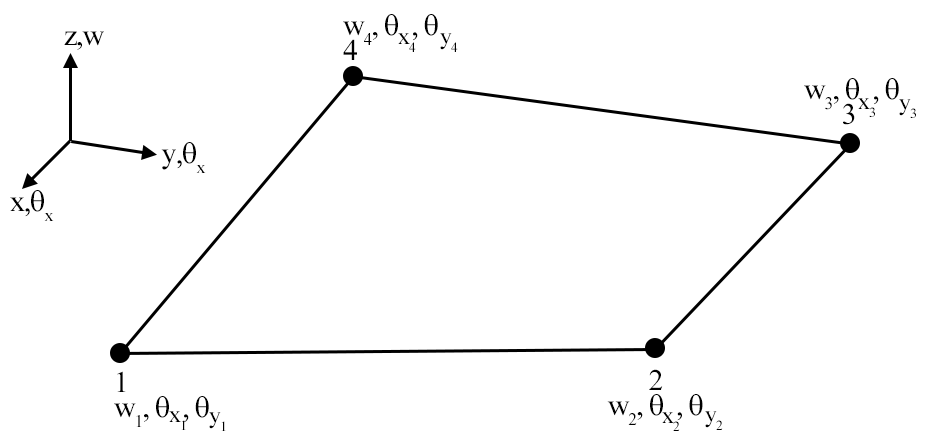
\includegraphics[width=0.97\linewidth]{figures/dkq}
  	\setlength\unitlength{1.0cm}
  	\begin{picture}(12.5,7)
  	\thicklines  
  	\put(1.5,4.5){\vector(0,1){1}}
  	\put(1.2,5.6){$z,w$}
  	\put(1.5,4.5){\vector(1,-0.2){1}}
  	\put(2.6,4.2){$y,\theta_y$}
  	\put(1.5,4.5){\vector(-0.5,-0.5){0.7}}
  	\put(0.6,3.5){$x,\theta_x$}
  	
  	\thinlines
  	\polyline(2.5,1.5)(8.5,1.6)(11.5,5)(5,6)(2.5,1.5)
  	\put(2.5,1.5){\circle*{0.25}}
  	\put(1.7,1.0){$w_1,\theta_{x_1},\theta_{y_1}$}
  	\put(8.5,1.6){\circle*{0.25}}
  	\put(7.8,1.1){$w_2,\theta_{x_2},\theta_{y_2}$}
  	\put(11.5,5){\circle*{0.25}}
  	\put(11.0,5.3){$w_3,\theta_{x_3},\theta_{y_3}$}
  	\put(5,6){\circle*{0.25}}
  	\put(4.2,6.3){$w_4,\theta_{x_4},\theta_{y_4}$}
  	\end{picture}
  	\caption{4-node quadrilateral plate element DKQ with 12 degrees-of-freedom, three per node.}
  	\label{fig:dkq}
  \end{figure}
  

  % dkq basiert auf diskretisierung der stress-energie, unter vernachlässigung der transverse shear strain energy (gl.(1) s.4)
  The formulation of the DKQ element by Batoz et al.~\cite{batoz1982evaluation} uses the discrete Kirchhoff technique. It is based on the discretization of the strain energy and neglects the transverse shear energy. This results in the following functional:
  \begin{equation}
  \Pi = \frac{1}{2} \int_A \vec{\kappa}^T \underline{D}_p \vec{\kappa}\ d\!A
  \end{equation}
  where $\underline{D}_p$ is the material matrix as defined previously (equation \eqref{eq:M=-Dp*kappa}) and $\vec{\kappa}$ denotes:
  \begin{equation}
  \vec{\kappa} = \begin{pmatrix}
  \frac{\partial \beta_x}{\partial x}\\
  \frac{\partial \beta y}{\partial y}\\
  \frac{\partial \beta_x}{\partial y} + \frac{\partial \beta_y}{\partial x}
  \end{pmatrix}
  \end{equation}
  $\beta_i$ is the rotation of the normal to the undeformed mid-surface in $x$-$z$-plane and $y$-$z$-plane, respectively. For $\Pi$ only $C^0$ continuity is required. Further,~\cite{batoz1982evaluation} states that $\beta_x$ and $\beta_y$ must be related to $w$ in such a way, that the final element satisfies the following requirements:
  \begin{itemize}
  	\item The nodal variables must be $w$, $\theta_x$ and $\theta_y$ with respect to $x$ and $y$ at the four element's nodes ($\theta_x = \partial w/\partial y, \theta_y=-\partial w/\partial x$)
  	\item The Kirchhoff boundary conditions must be satisfied.
  \end{itemize}
      
  % krümmungsvektor, Db angeben 
  % considerations für dkq formulierung
  Two incomplete cubic polynomial expressions define $\beta_x$ and $\beta_y$:
  \begin{align}
  \beta_x &= \sum_{i=1}^{8} N_i \beta_{x_i}\\
  \beta_y &= \sum_{i=1}^{8} N_i \beta_{y_i}
  \end{align}
  Here, $N_i(\xi,\eta)$ are the shape functions with isoparametric coordinates $\xi$ and $\eta$. They are the same as of the ``eight-node Serendipity'' element, described for example in~\cite{zienkiewicz2000finite}, or~\cite{braess2007finite} and seen in Figure~\ref{fig:serendipity}. The shape functions of this element are achieved by products of linear Lagrangian polynomials of the form $\frac{1}{4}(\xi+1)(\eta+1)$. For the eight-node element the following shape functions result:
  \begin{align}
  N_1(\xi, \eta) &= \frac{1}{4}(1-\xi)(1-\eta)(-\xi-\eta-1) \nonumber\\
  N_2(\xi, \eta) &= \frac{1}{4}(1+\xi)(1-\eta)(\xi-\eta-1) \nonumber\\
  N_3(\xi, \eta) &= \frac{1}{4}(1+\xi)(1+\eta)(\xi+\eta-1) \nonumber\\
  N_4(\xi, \eta) &= \frac{1}{4}(1-\xi)(1+\eta)(-\xi+\eta-1) \nonumber\\
  N_5(\xi, \eta) &= \frac{1}{2}(1-\xi^2)(1-\eta) \nonumber\\
  N_6(\xi, \eta) &= \frac{1}{2}(1+\xi)(1-\eta^2) \nonumber\\
  N_7(\xi, \eta) &= \frac{1}{2}(1-\xi^2)(1+\eta) \nonumber\\
  N_8(\xi, \eta) &= \frac{1}{2}(1-\xi)(1-\eta^2) \nonumber
  \end{align}
  \begin{figure}[htbp] % Bild 8.9 (a)~\cite{zienkiewicz2000finite}
  	\centering
  	%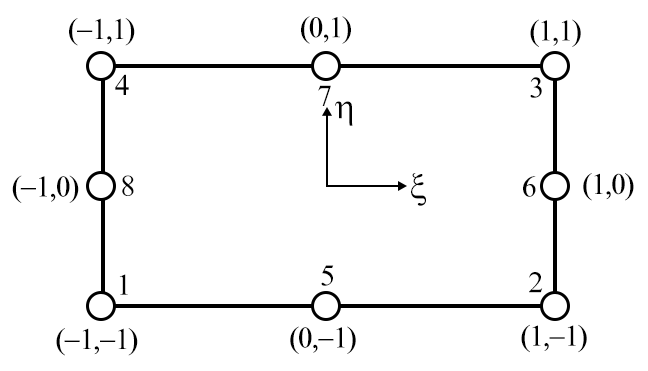
\includegraphics[width=0.97\linewidth]{figures/serendipity}
  	\setlength\unitlength{1.5cm}
  	\begin{picture}(8,5)
  	\thicklines  
  	\polyline(1.5,0.75)(1.5,4.25)(7,4.25)(7,0.75)(1.5,0.75)
  	\put(1.5,0.75){\circle*{0.2}}
  	\put(1.5,4.25){\circle*{0.2}}
  	\put(7,4.25){\circle*{0.2}}
  	\put(7,0.75){\circle*{0.2}}
  	\put(4.25,0.75){\circle*{0.2}}
  	\put(4.25,4.25){\circle*{0.2}}
  	\put(1.5,2.5){\circle*{0.2}}
  	\put(7,2.5){\circle*{0.2}}
  	
  	\thinlines
  	\put(4.25,2.5){\vector(1,0){1.25}}
  	\put(4.25,2.5){\vector(0,1){1.25}}
  	\put(5.3,2.2){$\xi$}
  	\put(4.4,3.5){$\eta$}
  	\put(1.1,4.5){$(-1,1)$}   \put(4.0,4.5){$(0,1)$}   \put(6.7,4.5){$(1,1)$}
  	\put(0.6,2.45){$(-1,0)$}                            \put(7.3,2.45){$(1,0)$}
  	\put(1.1,0.3){$(-1,-1)$}  \put(3.9,0.3){$(0,-1)$}  \put(6.7,0.3){$(1,-1)$}
  	
  	\put(1.7,3.9){$4$}  \put(4.2,3.9){$7$}  \put(6.6,3.9){$3$}
  	\put(1.7,2.4){$8$}                       \put(6.6,2.4){$6$}
  	\put(1.7,0.9){$1$}  \put(4.2,0.9){$5$}  \put(6.6,0.9){$2$}
  	\end{picture}
  	\caption{Eight-node quadrilateral element (``Seredipity''-element) with local $\xi,\eta$-~coordinates.}
  	\label{fig:serendipity}
  \end{figure}
  $\beta_{x_i}$ and $\beta_{y_i}$ are transitory nodal variables at the four nodes and mid-sides of the element.
  Next, Batoz et al. described the Kirchhoff assumptions at the corner nodes (cf. Figure~\ref{fig:serendipity} for the following):
  \begin{align}
  \begin{pmatrix}
  \beta_{x_i} + \partial w/\partial x_i \\
  \beta_{y_i} + \partial w/\partial y_i
  \end{pmatrix} = \begin{pmatrix}
  0\\0
  \end{pmatrix},\qquad i = 1,2,3,4
  \end{align}
  and at the mid-nodes:
  \begin{align}
  \beta_{s_k} + \partial w/\partial s_k = 0,\qquad k = 5,6,7,8
  \end{align}
  where $s$ denotes the coordinate along the element boundary and $\partial w/\partial s_k$ is the derivative of the displacement $w$ with respect to the mid-node $k$:
  \begin{equation}
  \frac{\partial w}{\partial s_k} = -\frac{3}{2 l_{ij}}(w_i-w_j) - \frac{1}{4}\left(\frac{\partial w}{\partial s_i} + \frac{\partial w}{\partial s_j}\right)
  \end{equation}
  with $k = 5,6,7,8$ being the mid-node of side $ij = 12, 23, 34, 41$ and $l_{ij}$ denotes the length of side $ij$.
  $\beta_n$ varies linearly along the sides:
  \begin{equation}
  \beta_{n_k} = \frac{1}{2}\left(\beta_{n_i} + \beta_{n_j}\right) = -\frac{1}{2} \left(\frac{\partial w}{\partial n_i} + \frac{\partial w}{\partial n_j}\right)
  \end{equation}
  with $k$ same as before.
  % formfunktionen, koeffizienten
  $\beta_x$ and $\beta_y$ can be rewritten as follows:
  \begin{align}
  \beta_x &= \vec{H}^x(\xi,\eta)^T \vec{w}\\
  \beta_y &= \vec{H}^y(\xi,\eta)^T \vec{w}\\
  \vec{w}^T &= \begin{pmatrix}
  w_1&\theta_{x_1}&\theta_{y_1}&w_2&\theta_{x_2}&\theta_{y_2}&w_3&\theta_{x_3}&\theta_{y_3}
  \end{pmatrix} \nonumber
  \end{align}
  with
  \begin{align}
  \vec{H}^{x^T} &= \begin{pmatrix}
  H_1^x & \dots & H_{12}^x
  \end{pmatrix} \nonumber\\
  H_{\left[1,4,7,10\right]}^x &= \frac{3}{2}\left(a_{\left[5,6,7,8\right]} N_{\left[5,6,7,8\right]} - a_{\left[8,5,6,7\right]} N_{\left[8,5,6,7\right]}\right) \nonumber\\
  H_{\left[2,5,8,11\right]}^x &= b_{\left[5,6,7,8\right]} N_{\left[5,6,7,8\right]} + b_{\left[8,5,6,7\right]} N_{\left[8,5,6,7\right]} \nonumber\\
  H_{\left[3,6,9,12\right]}^x &= N_{\left[1,2,3,4\right]} - c_{\left[5,6,7,8\right]} N_{\left[5,6,7,8\right]} - c_{\left[8,5,6,7\right]} N_{\left[8,5,6,7\right]} \nonumber\\
  \vec{H}^{y^T} &= \begin{pmatrix}
  H_1^y & \dots & H_{12}^y
  \end{pmatrix} \nonumber\\
  H_{\left[1,4,7,10\right]}^y &= \frac{3}{2}\left(d_{\left[5,6,7,8\right]} N_{\left[5,6,7,8\right]} - d_{\left[8,5,6,7\right]} N_{\left[8,5,6,7\right]}\right) \nonumber\\
  H_{\left[2,5,8,11\right]}^y &= -N_{\left[1,2,3,4\right]} + e_{\left[5,6,7,8\right]} N_{\left[5,6,7,8\right]} + e_{\left[8,5,6,7\right]} N_{\left[8,5,6,7\right]} \nonumber\\
  H_{\left[3,6,9,12\right]}^y &= -b_{\left[5,6,7,8\right]} N_{\left[5,6,7,8\right]} - b_{\left[8,5,6,7\right]} N_{\left[8,5,6,7\right]} \nonumber
  \end{align}
  The function notation $\bullet_{\left[i,j,k,l\right]}$ groups four functions together. The first function of the group gets the first index of the squared brackets, the second function the second index, and so on. The coefficients $a,b,c,d$ and $e$ are as follows:
  \begin{align}
  a_k &= -\frac{x_{ij}}{l_{ij}^2} \nonumber\\
  b_k &= \frac{3}{4} \frac{x_{ij} y_{ij}}{l_{ij}^2} \nonumber\\
  c_k &= \frac{ \frac{x_{ij}^2}{4} - \frac{y_{ij}^2}{2} }{l_{ij}^2} \nonumber\\
  d_k &= -\frac{y_{ij}}{l_{ij}^2} \nonumber\\
  e_k &= \frac{ \frac{y_{ij}^2}{4} - \frac{x_{ij}^2}{2} }{l_{ij}^2} \nonumber
  \end{align}
  where $k = 5,6,7,8$ for the sides $ij = 12, 23, 34, 41$, $x_{ij} = x_i - x_j$, $y_{ij} = y_i - y_j$ and $l_{ij}^2 = x_{ij}^2 + y_{ij}^2$. For more details about the derivation of these coefficients and functions $H^x$ and $H^y$ see~\cite{batoz1982evaluation}.
  
  % jacobi-matrix, -inverse, determinante
  Next, the Jacobian matrix $\underline{J}$ can be assembled, that is:
  \begin{equation}
  \underline{J} = \frac{1}{4} \begin{pmatrix}
  (x_{12}+x_{34})\eta - x_{12} + x_{34} & (y_{12} + y_{34})\eta - x_{12} + y_{34}\\
  (x_{12}+x_{34})\xi  - x_{13} - x_{24} & (y_{12} + y_{34})\xi  - y_{13} + y_{24}
  \end{pmatrix} = \begin{pmatrix}
  J_{11} & J_{12}\\ J_{21} & J_{22}
  \end{pmatrix}
  \end{equation}
  With its determinant $\left|\underline{J}\right|$ and inverse $\underline{J}^{-1}$:
  \begin{align}
  \left|\underline{J}\right| &= J_{11} J_{22} - J_{12} J_{21}\\
  \underline{J}^{-1} &= \frac{1}{\left|\underline{J}\right|} \begin{pmatrix}
  J_{22} & -J_{12}\\ -J_{21} & J_{11}
  \end{pmatrix} = \begin{pmatrix}
  j_{11} & j_{12}\\ j_{21} & j_{22}
  \end{pmatrix}
  \end{align}
  
  % krümmungs-verschiebungs-beziehung
  The strain-displacement matrix can now be obtained:
  \begin{equation}
  \underline{B} = \begin{pmatrix}
  \vec{H_x^x}\\\vec{H_y^y}\\\vec{H_y^x}+\vec{H_x^y}
  \end{pmatrix} = \begin{pmatrix}
  j_{11} & j_{12} & 0 & 0\\
  0 & 0 & j_{21} & j_{22}\\
  j_{21} & j_{22} & j_{11} & j_{12}\\
  \end{pmatrix} \begin{pmatrix}
  \vec{H_\xi^x}\\\vec{H_\eta^x}\\\vec{H_\xi^y}\\\vec{H_\eta^y}
  \end{pmatrix}
  \end{equation}
  The expressions $\vec{H_\xi^x}, \vec{H_\eta^x}, \vec{H_\xi^y}$ and $\vec{H_\eta^y}$ are vectors containing the derivatives of the corresponding components of the vectors $\vec{H^x}$ and $\vec{H^y}$ with respect to $\xi$ and $\eta$. The matrix $\underline{B}$ can then be inserted into the displacement-strain relation, like equation \eqref{eq:kappa=YBw}:
  \begin{equation}
  \vec{\kappa} = \underline{B} \vec{w}
  \end{equation}
  
  % steifigkeitsmatrix
  Next, $\vec{\kappa} = \underline{B} \vec{w}$ can be used in the functional to get the first term like equation \eqref{eq:t3_pi1=0.5wTKw}:
  \begin{align}
  \Pi_1 &= \frac{1}{2} \int_A \vec{\kappa}^T \underline{D}_p \vec{\kappa}\ d\!A \nonumber\\
  &= \frac{1}{2} \vec{w}^T \int_A \underline{B}^T \underline{D}_p \underline{B}\ d\!A \vec{w}\nonumber\\
  &= \frac{1}{2} \vec{w}^T \underline{K} \vec{w} \nonumber
  \end{align}
  with the stiffness matrix $\underline{K}$ of the DKQ element:
  \begin{align}
  \underline{K} &= \int_A \underline{B}^T \underline{D}_p \underline{B}\ d\!A \nonumber\\
  &= \int_{-1}^{1} \int_{-1}^{1} \underline{B}^T \underline{D}_p \underline{B}\ \left|\underline{J}\right|\ d\,\!\xi d\,\!\eta
  \end{align}
  
  The stiffness matrix can be numerically integrated with a $2\!\times\!2$ Gaussian integration scheme. Batoz et al. states that four sampling points are enough, although a $3\!\times\!3$ point scheme would be necessary for exact integration on a rectangular element~\cite{batoz1982evaluation}. Those four Gauss points are located at $\xi_i = \pm \frac{\sqrt{3}}{3}$ and $\eta_i = \pm \frac{\sqrt{3}}{3}$ with weight factor $\omega_i = 1$ equivalent to all four. The equation for the stiffness matrix can then be written in discretized form as follows:
  \begin{equation}
  \underline{K} = \sum_{i=1}^{2} \sum_{j=1}^{2} \omega_i \omega_j \underline{B}(\xi_i,\eta_j)^T \underline{D}_p \underline{B}(\xi_i,\eta_j) \left|\underline{J}(\xi_i,\eta_j)\right|
  \end{equation}
  When all nodal values $\vec{w}$ are known, the moments $\vec{M}$ at point $(x,y)$ in the element can be calculated:
  \begin{equation}
  \vec{M}(x,y) = \underline{D}_p \underline{B}(x,y) \vec{w}
  \end{equation}
  with
  \begin{equation}
  \vec{M} = \begin{pmatrix}
  M_x\\M_y\\M_{xy}
  \end{pmatrix}
  \end{equation}
 
 \subsection{Coordinate Transformation} \label{sec:Shell-CoTrafo}
  %see~\cite{nguyen2008smoothed}; genau:~\cite{zienkiewicz2000finite}\\
  The nodes and elements in the mesh are defined in a global three dimensional coordinate system. The elements need to be transformed into a two dimensional local coordinate system in order to be able to construct their local stiffness matrices. This local stiffness matrix must then be transformed back into the global system before adding it to the global stiffness matrix. This section describes the building of the transformation matrix, that will be used in the following section for the addressed transformation steps.
  First the transformation of an arbitrary triangle defined in 3D space is described. 
  
  \begin{figure}[htbp] % Bild von Dreieck mit ABC, globalem KoSys, lokalem KoSys mit Ursprung in A, x-Achse auf Vektor AB usw.\newline
  	\centering
  	%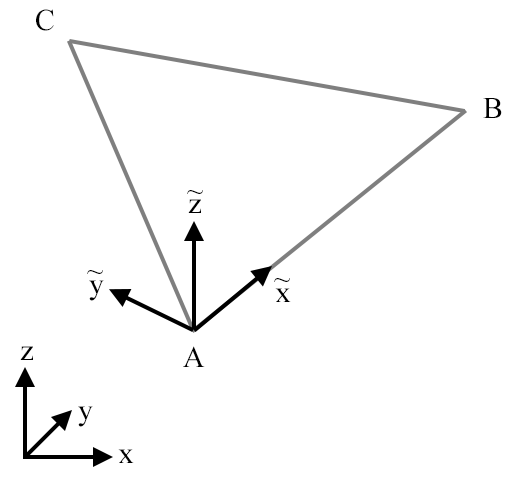
\includegraphics[width=0.4\linewidth]{figures/triangle}
  	\setlength\unitlength{0.80cm}
  	\begin{picture}(7.5,7.5)
  	\thicklines
  	\put(0,0){\vector(0,1){1}}
  	\put(1.1,0){$x$}
  	\put(0,0){\vector(1,0){1}}
  	\put(0,1.1){$z$}
  	\put(0,0){\vector(1,1){0.5}}
  	\put(0.6,0.6){$y$}      
  	\put(1.75,1.75){\vector(1,0.75){0.8}}
  	\put(2.65,1.95){$\tilde{x}$}
  	\put(1.75,1.75){\vector(-1,0.3){0.9}}
  	\put(0.55,1.75){$\tilde{y}$}
  	\put(1.75,1.75){\vector(0,1){1.0}}
  	\put(1.65,2.85){$\tilde{z}$}
  	\thinlines
  	\polyline(1.75,1.75)(7,5.8)(0.5,7)(1.75,1.75)
  	\put(1.5,1.3){$A$}
  	\put(7.20,5.7){$B$}
  	\put(0.0,6.9){$C$}
  	\end{picture}
  	\caption{Arbitrary triangle with nodes A, B and C, defined in global $xyz$-coordinate system. After transformation a new, local, $\tilde{x}\tilde{y}\tilde{z}$-coordinate system with node A in its origin, is created.}
  	\label{fig:triangle}
  \end{figure}
    
  Given a triangle with vertices $\vec{A} = (a_x, a_y, a_z)^T, \vec{B} = (b_x, b_y, b_z)^T$ and $\vec{C} = (c_x, c_y, c_z)^T$ ordered in counterclockwise direction, as shown in Figure~\ref{fig:triangle}. Let $\vec{u}$ be the vector from node $\vec{A}$ to $\vec{B}$ and $\vec{v}$ be the vector from node $\vec{A}$ to $\vec{C}$:
  \begin{align*}
  \vec{u} &= \vec{B}-\vec{A} = \begin{pmatrix}
  b_x - a_x & b_y - a_y & b_z - a_z
  \end{pmatrix}^T\\
  \vec{v} &= \vec{C}-\vec{A} = \begin{pmatrix}
  c_x - a_x & c_y - a_y & c_z - a_z
  \end{pmatrix}^T
  \end{align*}
  First local unit vector:
  \begin{equation*}
   \vec{\tilde{x}} = \frac{1}{\left|\vec{u}\right|}\vec{u}
  \end{equation*}
  Second local unit vector:
  \begin{align*}
   \vec{\tilde{z}} &= \vec{u} \times \vec{v} \\
   \vec{\tilde{z}} &\leftarrow \frac{1}{\left|\vec{\tilde{z}}\right|}\vec{\tilde{z}}
  \end{align*}
  Third local unit vector:
  \begin{equation*}
   \vec{\tilde{y}} = \vec{\tilde{z}} \times \vec{\tilde{x}}
  \end{equation*}
  Define transformation matrix $\underline{T}$ as follows:
  \begin{equation}\label{eq:trafoT_tri}
   \underline{T} = \begin{pmatrix}
   \vec{\tilde{x}}^T\\ \vec{\tilde{y}}^T\\ \vec{\tilde{z}}^T
   \end{pmatrix} = \begin{pmatrix}
   \tilde{x}_x & \tilde{x}_y & \tilde{x}_z\\
   \tilde{y}_x & \tilde{y}_y & \tilde{y}_z\\
   \tilde{z}_x & \tilde{z}_y & \tilde{z}_z
   \end{pmatrix}
  \end{equation}
  Assembly of element's stiffness matrix needs partial derivatives. In order to get these derivatives with less computational effort, every triangle can be translated in such a way, that node $\vec{A}$ lies in the global origin before transforming it to local coordinates. Node $\vec{A}$ stays at $(0,\ 0,\ 0)$ coordinates which then simplifies getting the derivatives (see Section~\ref{sec:Impl-Details-Assembly}). It follows:
  \begin{align*}
   \vec{\tilde{A}} &= \begin{pmatrix}
   0 & 0 & 0
   \end{pmatrix}^T \\
   \vec{\tilde{B}} &= \begin{pmatrix}
   \tilde{b}_x & 0 & 0
   \end{pmatrix}^T \\
   \vec{\tilde{C}} &= \begin{pmatrix}
   \tilde{c}_x & \tilde{c}_y & 0
   \end{pmatrix}^T
  \end{align*}
  Node $\vec{A}$ will not be changed by the transformation with $\underline{T}$, $\vec{B}$ will be projected onto the local $x$-axis that is defined to be the normalized vector between $\vec{A}$ and $\vec{B}$. Node $\vec{C}$ will be projected onto the local $xy$-plane. One can see that the $z$-component vanishes by transforming into local space, thus generating the two dimensional local space.
  
  \begin{figure}[htbp] % Bild von bel. Viereck mit ABCD, IJKL, globalem KoSys, lokalem KoSys mit Ursprung auf Schnittpunkt der gestrichelten Linien von JL und IK\newline
  	\centering
  	%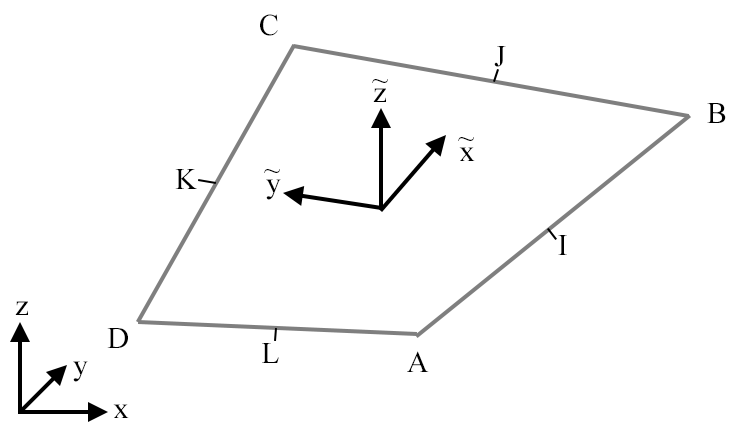
\includegraphics[width=0.5\linewidth]{figures/quadrilateral}
  	\setlength\unitlength{0.99cm}
  	\begin{picture}(7,5)
  	\thicklines
  	\put(0,0){\vector(0,1){1}}
  	\put(1.1,0){$x$}
  	\put(0,0){\vector(1,0){1}}
  	\put(0,1.1){$z$}
  	\put(0,0){\vector(1,1){0.5}}
  	\put(0.6,0.6){$y$}
  	\put(3.4,2.35){\vector(0.45,0.75){0.6}}
  	\put(4.1,3.0){$\tilde{x}$}
  	\put(3.4,2.35){\vector(-0.9,0.2){0.9}}
  	\put(2.25,2.65){$\tilde{y}$}
  	\put(3.4,2.35){\vector(0,1){1.0}}
  	\put(3.3,3.45){$\tilde{z}$}
  	\thinlines
  	\polyline(1,1)(4,0.5)(6.5,3.5)(2,4.5)(1,1)
  	\put(0.5,0.9){$D$}
  	\put(3.9,0){$A$}
  	\put(6.6,3.3){$B$}
  	\put(1.6,4.5){$C$}
  	\put(2.25,0.2){$L$}
  	\put(1.0,2.55){$K$}
  	\put(4.2,4.2){$J$}
  	\put(5.45,1.7){$I$}
  	\unitlength=0.99mm
  	\Dline(25,7.5)(43,40){1.5}
  	\Dline(52,19.5)(15,27.0){1.5}
  	\end{picture}
  	\caption{Quadrilateral with nodes A, B, C and D, defined in global $xyz$ coordinate system. After transformation a new, local, $\tilde{x}\tilde{y}\tilde{z}$ coordinate system is created.}
  	\label{fig:quadrilateral}
  \end{figure}
  
  The other element described in this work is the quadrilateral. Let an arbitrary quadrilateral be given with vertices $\vec{A} = (a_x,\ a_y,\ a_z)^T, \vec{B} = (b_x,\ b_y,\ b_z)^T, \vec{C} = (c_x,\ c_y,\ c_z)^T, \vec{D} = (d_x,\ d_y,\ d_z)^T$ ordered in counterclockwise direction, cf. Figure~\ref{fig:quadrilateral}. Next, let $\vec{I}$ be the midpoint of edge $\overline{AB}$:
  \begin{equation*}
   \vec{I} = \vec{A} + \frac{1}{2}\left( \vec{B}-\vec{A}\right)
  \end{equation*}
  Analogously let $\vec{J}, \vec{K}$ and $\vec{L}$ be the midpoints of the edges $\overline{BC}, \overline{CD}$ and $\overline{DA}$:
  \begin{align*}
   \vec{J} &= \vec{B} + \frac{1}{2}\left( \vec{C}-\vec{B}\right) \\
   \vec{K} &= \vec{C} + \frac{1}{2}\left( \vec{D}-\vec{C}\right) \\
   \vec{L} &= \vec{D} + \frac{1}{2}\left( \vec{A}-\vec{D}\right)
  \end{align*}
  Let then $\vec{u}$ be the vector from node $\vec{L}$ to $\vec{J}$ and $\vec{v}$ be the vector from node $\vec{I}$ to $\vec{K}$:
  \begin{align*}
   \vec{u} &= \vec{J}-\vec{L} = \begin{pmatrix}
   j_x-l_x & j_y-l_y & j_z-l_z
   \end{pmatrix}^T\\
   \vec{v} &= \vec{K}-\vec{I} = \begin{pmatrix}
   k_x-i_x & k_y-i_y & k_z-i_z
   \end{pmatrix}^T
  \end{align*}
  First local unit vector:
  \begin{equation*}
   \vec{\tilde{x}} = \frac{1}{\left|\vec{u}\right|}\vec{u}
  \end{equation*}
  Second local unit vector:
  \begin{align*}
   \vec{\tilde{z}} &= \vec{u} \times \vec{v}\\
   \vec{\tilde{z}} &\leftarrow \frac{1}{\left|\vec{\tilde{z}}\right|}\vec{\tilde{z}}
  \end{align*}
  Third local unit vector:
  \begin{equation*}
   \vec{\tilde{y}} = \vec{\tilde{z}} \times \vec{\tilde{x}}
  \end{equation*}
  Define transformation matrix $T$ as follows:
  \begin{equation}\label{eq:trafoT_quad}
   \underline{T} = \begin{pmatrix}
   \vec{\tilde{x}}^T\\ \vec{\tilde{y}}^T\\ \vec{\tilde{z}}^T
   \end{pmatrix} = \begin{pmatrix}
   \vec{\tilde{x}}_x & \vec{\tilde{x}}_y & \vec{\tilde{x}}_z\\ \vec{\tilde{y}}_x & \vec{\tilde{y}}_y & \vec{\tilde{y}}_z\\ \vec{\tilde{z}}_x & \vec{\tilde{z}}_y & \vec{\tilde{z}}_z
   \end{pmatrix}
  \end{equation}
  Remark: In order to transform a quadrilateral element from 3D to a local two dimensional space, the nodes of the original element must all be located on a common plane. Otherwise such a transformation cannot be performed. Such shaped quadrilaterals cannot be used as shell elements.
 
 
 \subsection{Shell Element}\label{sec:Shell-Shell}
 % The combination of the two previous parts and the transformations results in the final shell element\newline
 Shell elements combine the capability of both, plane and plate elements. Every time a thin walled structure like a car body, dome structure or container with multi-axial pressures is to be simulated, shell elements provide a good solution. In this work only the so-called flat shell elements are described and used in the implementation. Details about curved shell elements, shells of revolution and general shells can be found in~\cite{cook2002concepts}.
 
 Flat shell elements have a state of bending and membrane stress that can be described by superposition of the plane and plate element~\cite{klein2013fem}. Figure~\ref{fig:shell_triangle} shows the superposition of plane and plate elements to a flat shell element. The degrees of freedom of plane and plate at every node are combined at the node of the shell element. Obviously the plane and plate element must be of the same finite element's type, for example three-node triangular or eight-node quadrilateral.
 \begin{figure}[htbp] % bild wie bei 8.7 von scheibe und platte und kombination zu schale + erklärungen, welche unbekannten und kräfte man bei welchem teil hat
 	\centering
 	%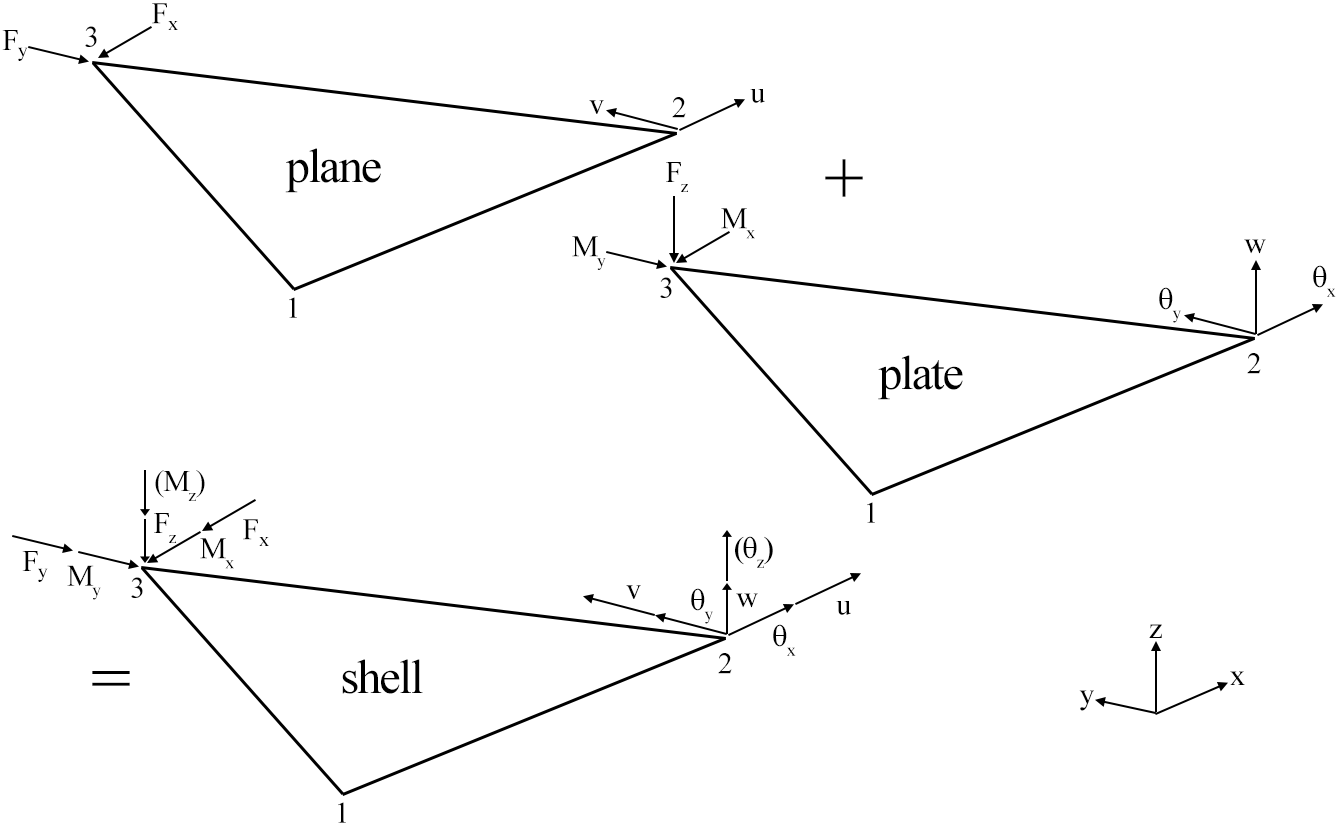
\includegraphics[width=0.8\linewidth]{figures/shell_triangle}
 	\setlength\unitlength{0.9cm}
 	\begin{picture}(11.5,9.5)
 	\thicklines
 	\put(10.0,3.5){\vector(1,0.5){0.55}}   \put(10.6,3.5){$x$}
 	\put(10.0,3.5){\vector(-0.5,1){0.25}}  \put(9.5,3.6){$y$}
 	\put(10.0,3.5){\vector(0,1){0.7}}      \put(9.9,4.3){$z$}
 	
 	\put(5.5,7.0){\vector(1,0.5){0.55}}   \put(6.0,6.9){$u$}
 	\put(5.5,7.0){\vector(-0.5,1){0.25}}  \put(4.8,7.3){$v$}
 	\put(1.55,8.8){\vector(-1,-0.5){0.55}}\put(1.4,8.45){$F_x$}
 	\put(0.7,9.0){\vector(0.5,-1){0.25}}  \put(0.3,8.45){$F_y$}
 	
 	\put(10.5,7.0){\vector(0,1){0.7}}     \put(10.6,7.3){$w$}
 	\put(10.5,7.0){\vector(1,0.5){0.55}}  \put(11.0,6.9){$\theta_x$}
 	\put(10.5,7.0){\vector(-0.5,1){0.25}} \put(9.8,7.3){$\theta_y$}
 	\put(6.0,9.2){\vector(0,-1){0.7}}     \put(6.1,8.9){$F_z$}
 	\put(6.55,8.8){\vector(-1,-0.5){0.55}}\put(6.4,8.45){$M_x$}
 	\put(5.7,9.0){\vector(0.5,-1){0.25}}  \put(5.3,8.45){$M_y$}
 	
 	\put(8.0,2.0){\vector(0,1){0.7}}      \put(8.1,2.3){$w$}
 	\put(8.0,2.0){\vector(1,0.5){0.55}}   \put(8.5,1.9){$\theta_x$}
 	\put(8.0,2.0){\vector(-0.5,1){0.25}}  \put(7.3,2.3){$\theta_y$}
 	\put(3.5,4.2){\vector(0,-1){0.7}}     \put(3.6,3.9){$F_z$}
 	\put(4.05,3.8){\vector(-1,-0.5){0.55}}\put(3.9,3.45){$M_x$}
 	\put(3.2,4.0){\vector(0.5,-1){0.25}}  \put(2.8,3.45){$M_y$}
 	\put(8.6,2.3){\vector(1,0.5){0.55}}   \put(9.0,2.2){$u$}
 	\put(7.75,2.5){\vector(-0.5,1){0.25}} \put(7.2,2.6){$v$}
 	\put(4.65,4.1){\vector(-1,-0.5){0.55}}\put(4.4,3.75){$F_x$}
 	\put(2.95,4.5){\vector(0.5,-1){0.25}} \put(2.6,3.9){$F_y$}
 	\put(8.0,2.7){\vector(0,1){0.7}}      \put(8.1,3.0){$(\theta_z)$}
 	\put(3.5,4.9){\vector(0,-1){0.7}}     \put(3.6,4.6){$(M_z)$}
 	\thinlines
 	\polyline(1.0,8.5)(2.5,5.5)(5.5,7.0)(1.0,8.5)
 	\put(2.3,5.1){$1$} \put(5.3,6.5){$2$} \put(0.8,8.0){$3$} 
 	\polyline(6.0,8.5)(7.5,5.5)(10.5,7.0)(6.0,8.5)
 	\put(7.3,5.1){$1$} \put(10.3,6.5){$2$} \put(5.8,8.0){$3$}  
 	\polyline(3.5,3.5)(5.0,0.5)(8.0,2.0)(3.5,3.5)
 	\put(4.8,0.1){$1$} \put(7.8,1.5){$2$} \put(3.3,3.0){$3$}
 	
 	\put(5.85,5.9){\textbf{{\Huge +}}} \put(2.3,1.5){\textbf{{\Huge =}}}
 	\put(2.5,6.7){\textbf{plane}}
 	\put(7.5,6.8){\textbf{plate}}
 	\put(5.1,1.7){\textbf{shell}}
 	\end{picture}
 	\caption{Creation of a triangular flat shell element by superimposing a triangular plane and a triangular plate element. The elements are described in the same local coordinate system with their degrees of freedom shown exemplary at one node per element.}
 	\label{fig:shell_triangle}
 \end{figure} 
 The plane has displacements $u$ and $v$ with dedicated forces $F_x$ and $F_y$. The plate has the deformation $w$ with assigned normal force $F_z$ and the two twists $\theta_x$ and $\theta_y$ with assigned moments $M_x$ and $M_y$. Through the linking of the elements the shell element node has now five natural degrees of freedom. An additional twist around the local z-axis $\theta_z$ will be introduced~\cite{steinke2005finite}, increasing the number to six degrees of freedom per node. In vector notation the resulting displacement vector $\vec{u}_i$ of a shell element's node $i$ is:
 \begin{align}\label{eq:shell_u_i}
 \vec{u} &= \underbrace{\begin{pmatrix}
 	u\\v\\w\\\theta_x\\\theta_y\\\theta_z
 	\end{pmatrix}} = \underbrace{\begin{pmatrix}
 	u\\v\\0\\0\\0\\0
 	\end{pmatrix}} + \underbrace{\begin{pmatrix}
 	0\\0\\w\\\theta_x\\\theta_y\\0
 	\end{pmatrix}} + \begin{pmatrix}
 0\\0\\0\\0\\0\\\theta_z
 \end{pmatrix}\\
 &\quad\;\; \text{shell}\ \quad\; \text{plane}\ \quad\! \text{plate}
 \end{align}
 
 % gesamtsteifigkeitsmatrix besteht aus blöcken (3x3 bei tri3, 4x4 bei quad4), Ku=F (gleichung 718 bei~\cite{steinke2005finite})
 For the two different finite elements in this work -- the three-node triangular element and the four-node quadrilateral element -- the stiffness matrix for the shell element is described by a block matrix of either $3\!\times\!3$ submatrices for the triangular case or $4\!\times\!4$ submatrices for the quadrilateral. The following equation shows the latter case as example:
 \begin{align}\label{eq:shell_K_ij}
 \underline{K} \vec{u} &= \vec{F} \nonumber\\
 \begin{pmatrix}
 \underline{K}_{11} & \underline{K}_{12} & \underline{K}_{13} & \underline{K}_{14}\\
 \underline{K}_{21} & \underline{K}_{22} & \underline{K}_{23} & \underline{K}_{24}\\
 \underline{K}_{31} & \underline{K}_{32} & \underline{K}_{33} & \underline{K}_{34}\\
 \underline{K}_{41} & \underline{K}_{42} & \underline{K}_{43} & \underline{K}_{44}
 \end{pmatrix} \begin{pmatrix}
 \vec{u}_1 \\\vec{u}_2 \\\vec{u}_3\\\vec{u}_4
 \end{pmatrix} &= \begin{pmatrix}
 \vec{F}_1\\\vec{F}_2\\\vec{F}_3\\\vec{F}_4
 \end{pmatrix}
 \end{align}
 where the vectors $\vec{u}_i$ are the same as in equation \eqref{eq:shell_u_i}. The single submatrices $\underline{K}_{ij}$ of $\underline{K}$ were created by the superposition of the stiffness matrices of the plane and the plate:
 \begin{equation}
 \underline{K}_{ij} = \left(\underline{\hat{K}}_{ij}\right)_m + \left(\underline{\hat{K}}_{ij}\right)_p
 \end{equation}
 The submatrix $\underline{K}_{ij}$ has the following structure:
 \begin{align}
 \begin{gmatrix}[p]
 \circ & \circ & 0     & 0     & 0     & 0 \\
 \circ & \circ & 0     & 0     & 0     & 0 \\
 0     & 0     & \star & \star & \star & 0 \\
 0     & 0     & \star & \star & \star & 0 \\
 0     & 0     & \star & \star & \star & 0 \\
 0     & 0     & 0     & 0     & 0     & 0
 \colops
 \mult{0}{u}
 \mult{1}{v}
 \mult{2}{w}
 \mult{3}{\theta_x}
 \mult{4}{\theta_y}
 \mult{5}{\theta_z}
 \rowops
 \mult{0}{u}
 \mult{1}{v}
 \mult{2}{w}
 \mult{3}{\theta_x}
 \mult{4}{\theta_y}
 \mult{5}{\theta_z}
 \end{gmatrix} &= \begin{gmatrix}[p]
 \circ & \circ & 0 & 0 & 0 & 0 \\
 \circ & \circ & 0 & 0 & 0 & 0 \\
 0     & 0     & 0 & 0 & 0 & 0 \\
 0     & 0     & 0 & 0 & 0 & 0 \\
 0     & 0     & 0 & 0 & 0 & 0 \\
 0     & 0     & 0 & 0 & 0 & 0
 \colops
 \mult{0}{u}
 \mult{1}{v}
 \mult{2}{w}
 \mult{3}{\theta_x}
 \mult{4}{\theta_y}
 \mult{5}{\theta_z}
 \rowops
 \mult{0}{u}
 \mult{1}{v}
 \mult{2}{w}
 \mult{3}{\theta_x}
 \mult{4}{\theta_y}
 \mult{5}{\theta_z}
 \end{gmatrix} + \begin{gmatrix}[p]
 0     & 0     & 0     & 0     & 0     & 0 \\
 0     & 0     & 0     & 0     & 0     & 0 \\
 0     & 0     & \star & \star & \star & 0 \\
 0     & 0     & \star & \star & \star & 0 \\
 0     & 0     & \star & \star & \star & 0 \\
 0     & 0     & 0     & 0     & 0     & 0
 \colops
 \mult{0}{u}
 \mult{1}{v}
 \mult{2}{w}
 \mult{3}{\theta_x}
 \mult{4}{\theta_y}
 \mult{5}{\theta_z}
 \rowops
 \mult{0}{u}
 \mult{1}{v}
 \mult{2}{w}
 \mult{3}{\theta_x}
 \mult{4}{\theta_y}
 \mult{5}{\theta_z}
 \end{gmatrix}
 \end{align}
 % Sei $K_m$ die lokale Steifigkeitsmatrix vom Membran/Plane-Teil und $K_p$ die vom Plate-bending-Teil
 
 % Kij weisst in der Spalte theta\_z und Zeile theta\_z $(k_ij)_66$ eine null auf -> erklärung und warum schlecht. ANDERE REFERENZ ERKLÄRT, WAS WIR DESHALB MACHEN (1/1000 der diagonalwerte)
 $\left(\underline{\hat{K}}_{ij}\right)_m$ describes the submatrix of the stiffness matrix of the plane element for node $i$ and $j$ and is marked with the $\circ$-symbol, $\left(\underline{\hat{K}}_{ij}\right)_p$ describes the corresponding matrix part of the plate element's stiffness matrix and is symbolized with a $\star$.
 The degree of freedom $\theta_z$ does not exists in both, the plane and the plate element, and is introduced with the shell element. Therefore $(\underline{K}_{ij})_{66}$ is zero. The sixth degree of freedom is necessary because the missing stiffness regarding a rotation around the axis normal to the element could produce singularities in the overall stiffness matrix. This happens for example, if all neighboring elements of a node lie in the same plane, i.e. they are coplanar. A singularity can lead to a non-solvable system, so this case needs be excluded~\cite{steinke2005finite}. One way is to introduce this sixth degree of freedom and give it a value that is so small that it does not influence the displacements and stresses too much. The number of this values varies: ~\cite{werkle1995finite} suggests a value of $1/10000$ of the smallest diagonal entry of $\underline{K}_{ij}$, whereas~\cite{kansara2004development} used $1/1000$ of the smallest diagonal entry of $\underline{K}_{ij}$. The value must be small, but big enough to prevent the singularities. Since this value is an approximation, one has to modify it, if the solution is not as expected or one cannot get a solution at all due to the addressed singularities.
 
 % Dann muss die (Rück-)Transformationsmatrix $T$ erstellt werden, da SKM im lokalen KoSys definiert ist, aber in die globale Systemmatrix einsortiert werden muss
 The stiffness matrix for the shell element was constructed in a local coordinate system as described in Section~\ref{sec:Shell-Plane},~\ref{sec:Shell-Plate} and~\ref{sec:Shell-CoTrafo}. The overall stiffness matrix contains information about all elements and needs to be described in a global coordinate system. Before the element stiffness matrix is added to the global stiffness matrix, it has to be transformed from local to global. This can be achieved by transforming the single blocks of $\underline{K}$ from equation \eqref{eq:shell_K_ij} with the relation:
 \begin{equation}\label{eq:shell_K_ij u_j=F_i}
 \underline{\check{K}}_{ij} \vec{\check{u}}_j = \vec{\check{F}}_i
 \end{equation}
 where ``\;$\check{\ }$\;'' denotes that the matrix and vector are represented in local coordinates. With the help of the transformation matrix $\underline{\tilde{T}}$, the globally described displacement vector $\vec{u}_j$ and load vector $\vec{F}_i$ can be represented in local coordinates:
 \begin{align}
 \check{\vec{u}}_j = \underline{\tilde{T}} \vec{u}_j\\
 \check{\vec{F}}_i = \underline{\tilde{T}} \vec{F}_i
 \end{align}
 Since the load vector is to be defined in a global coordinate system and the resulting displacements are to be defined globally, too, equation \eqref{eq:shell_K_ij u_j=F_i} will be multiplied by $\underline{\tilde{T}}^T$ from left:
 \begin{equation}
 \underline{\tilde{T}}^T \underline{\check{K}}_{ij} \underline{\tilde{T}} \vec{u}_j = \underline{\tilde{T}}^T \underline{\tilde{T}} \vec{F}_i = \vec{F}_i
 \end{equation}
 Hence, the two vectors will be represented in global coordinates and only the local element stiffness matrix need to be transformed. The addressed $6\!\times\!6$ transformation matrix $\underline{\tilde{T}}$ is made up of the $3\!\times\!3$ transformation matrix $\underline{T}$ from Section~\ref{sec:Shell-CoTrafo}:
 \begin{equation}\label{eq:trafoTtilde}
 \underline{\tilde{T}} = \begin{pmatrix}
 \underline{T} & 0\\
 0 & \underline{T}
 \end{pmatrix}
 \end{equation}
 
 % Je nachdem ob 3 oder 4 Knotenelement (Tri-3/Quad-4) sieht $K$ und $T$ natürlich anders aus
 In order to get the local element stiffness matrix $\underline{K}$ transformed to the global coordinate system, one has to transform the single submatrices $\underline{K}_{ij}$ as follows:
 \begin{equation}\label{eq:Kij=Tt Kij T}
 \underline{K}_{ij} = \underline{\tilde{T}}^T \underline{\check{K}}_{ij} \underline{\tilde{T}}
 \end{equation}
 for $1 \leq i,j \leq 3$ in the case of the triangular element and $1 \leq i,j, \leq 4$ for the quadrilateral element, respectively.